\documentclass[12pt,a4paper,notitlepage]{article}
\usepackage[utf8]{inputenc}
\usepackage[english]{babel}
\usepackage[T1]{fontenc}
\usepackage[affil-it]{authblk}
\usepackage[backend=biber,
			style=authoryear-icomp,
			sortlocale=de_DE,
			natbib=true,
			isbn=false,
			doi=false,
			bibstyle=authoryear,
			]{biblatex}
\usepackage{eurosym}
\usepackage{enumitem}
\usepackage{url}
\usepackage{blindtext}
\usepackage{hyperref}
\usepackage{breakurl}
\usepackage{amsmath}
\usepackage{titling}
\usepackage{amsfonts}
\usepackage{amssymb}
\usepackage{pgfplots}
\usepackage{caption}
\usepackage{subcaption}
\usepackage{graphicx}
\usepackage{dcolumn}
\usepackage{tikz-3dplot}
\usepackage{subcaption}
\usepackage{float}
\usepackage{adjustbox}
\usepackage{multirow,rotating}
\usepackage[autostyle]{csquotes}
\usepackage[toc,page]{appendix}
\usepackage{lscape}
\usepackage{todonotes}
\usepackage{booktabs}
\usepackage{multirow}
\usepackage{bm}
\usepackage{eurosym}
\usepackage{pdflscape}
\usepackage{geometry}
\geometry{a4paper,left=30mm,right=20mm, top=2cm, bottom=2cm} 

\addbibresource{Textmining.bib}
\ExecuteBibliographyOptions{maxcitenames=2,mincitenames=1}
\renewcommand*{\mkbibnamelast}[1]{\textsc{#1}}

\title{Topic and tone of political news articles in German online media.}
\date{\today}

\author{Franziska Löw
  \thanks{Electronic address: \texttt{loewf@hsu-hh.de}}}
\affil{Department of Industrial Economics,\\ Helmut Schmidt University,\\ Hamburg, Germany}

\begin{document}
\begin{titlepage}
	\maketitle
	\begin{abstract}
	However, the concept of media bias actually encompasses different subtypes: Visibility bias is the salience of political actors, tonality bias the evaluation of these actors, and agenda bias the extent to which parties address preferred issues in media coverage. Most literature on media bias focuses on only one type of bias, mainly disregarding agenda bias, as the operationalization is somewhat challenging. Additionally, studies that analyse the effect of media content primarily employ manual content analysis and are therefore much more time-consuming and susceptible to errors. Using automated data mining tools this paper provides an approach that allows an efficient and objective analysis to measure the different types of media bias. In order to investigate whether the media landscape transmits a biased reality of the political landscape, online news articles are analysed together with party press releases.
	\end{abstract}

\end{titlepage}

\tableofcontents

\pagebreak

%------------------------------------------------%
%----------------- Begin paper -------------------%
%------------------------------------------------%

\section{Introduction}

The discussion about the influence of digital media on the political opinion-forming process has gained momentum since the presidential elections in October 2016. The importance of the internet as a source of information for political topics has grown strongly in recent years. Even though television remains the most widely used source of news in Germany (2018: 74\%), numbers watching continue to decline while use of the internet for news has grown significantly in the last year (+5\%, 2018: 65\%) \citep{holig_reuters_2018}. The expansion of the internet as a new method of communication provides a potential challenge to the primacy of the traditional media and political parties as formers of public opinion \citep{savigny_public_2002}.

However, the influence of media bias on voter preferences has not only been studied in the literature since the growing importance of the internet. The general hypothesis is that bias in political news may have a profound influence on voter opinions and preferences \citep{ferree_four_2002, mccombs_look_2005, eberl_one_2017}. It can therefore be argued, that one central responsibility of the media is to supply voters with balanced and objective information on relevant political issues and actors \citep{stromback_four_2008, eberl_one_2017}. However, the concept of media bias actually encompasses different subtypes \citep{dalessio_media_2000, eberl_one_2017, junque_de_fortuny_media_2012}: (1) Coverage bias, (2) tonality bias und (3) agenda bias. These three concepts measure how often political actors appear in the media (coverage bias), how they are evaluated (tonality bias) and whether they are able to present their own political positions and talk about their issues in the media (agenda bias). The latter therefore stems from a journalist's or editor's decision to select or ignore specific news stories. Most of the literature on media bias focuses on one type of bias and most research tends to disregard agenda bias as the operationalization is somewhat more challenging. In order to know which news stories have been selected as well as deselected by journalists, one would have to know the universe of news stories at a given point in time \citep{dalessio_media_2000}. I adopt the approach used in \citet{eberl_one_2017}, in using parties' campaign communication as an approximation of the potential universe of news stories. However, this analysis differs from earlier approaches in that I use machine learning techniques to identify the underlying topics in the text corpus. Furthermore, I use text-mining techniques to measure coverage and tonality bias. Similar to \citet{junque_de_fortuny_media_2012} I refrained from interpreting the results on a political level as much as possible, yet I demonstrate how text-mining techniques allow an efficient and objective analysis of today's on-line media landscape. 

The data analyzed in this study contains nearly 12.000 online news articles from seven major news provider dated from June 1, 2017 to March 1, 2018 as well as over 1.900 press releases of the parties in the german "Bundestag". As the German federal elections took place on 24th of September 2017 and the formation of the government has taken up a period of about five months, the articles considered inform their readers about both the election promises of the parties (before the election) and the coalition talks (after the election). 

% --- coverage bias --- %

% --- sentiament bias --- %

To conduct such an analysis, a list of words (dictionary) associated with a given emotion, such as negativity is pre-defined. The document is then deconstructed into individual words and each word is assigned a sentiment value according to the dictionary, where the sum of all values results in the emotional score for the given document. 

% --- agenda bias --- %

While the coverage and tonality bias can be calculated using simple counting methods, more sophisticated approaches are required to operationalize the agenda bias, since the topics covered have to be identified. To discover the latent topics in the corpus of text data, the structural topic modeling (STM) developed by \citet{roberts_model_2016} is applied. The STM is an unsupervised machine learning approach that models topics as multinomial distributions of words and documents (as a synonym for news articles) as multinomial distributions of topics, allowing the incorporation of external variables that affect both, topical content and topical prevalence. The results of the generative process of the STM are two posterior distributions: One for the topic prevalence in a document (what is the article or press release about?) and one for the content of a topic (what is the topic about?).

% --- Key contributions --- %

Building on the insight that media bias can have three different forms, this study makes two key contributions. (1) combination of different text-mining techniques to analyze a large text corpus reduces the human induced bias and makes research more traceable and comparable. Our measures of media bias are based on extensive content analyses of newspaper coverage and party press releases. and (2) a new approach to measure agenda bias.    

This study presents evidence from an integrated research design that combines data from an extensive media content analysis of eight national newspapers with data about party press releases of six parties

% --- remaining course of the paper... --- %

The remaining course of the paper is as follows: The following section provides an overview of the related literature. Section \ref{ch_elections} gives a introduction to the political trends in the past six month (June 2017 to March 2018). The data used to conduct the model is described in section \ref{ch_data}. Section \ref{ch_model} explains the generative process of the structural topic model as well as the selected parameters to run the model. The empirical analysis is conducted in section \ref{ch_empirical}. 

%-------------------------------------------------------%
%----------------- Literature Review -------------------%
%-------------------------------------------------------%

\section{Literature}

Most of the literature on influences of media bias focuses on one type of bias (see \citet{eberl_one_2017}). Overall, most research tends to disregard agenda bias as the operationalization is somewhat more challenging. In order to know which news stories have been selected as well as deselected by journalists, one would have to know the universe of news stories at a given point in time \citet{dalessio_media_2000}. \citet{eberl_one_2017} use parties' campaign communication as an approximation of the potential universe of news stories \citep{brandenburg_political_2005}

So kann beispielsweise eine stärkere Verbreitung von politischen Inhalten einer Partei einen positiven Einfluss auf die Einstellung gegenüber dieser Partei haben \citep{benewick_floating_1969}. Vor der Annahme, dass Medien einen Einfluss auf Wählerpräferenzen haben, werfen \citet{mccombs_agenda-setting_1972} die Frage auf, ob die politische Welt in den Medien unverzerrt abgebildet wird. Sie kommen zu dem Ergebnis, dass Massenmedien die politische Agenda beeinflusst. 

%---- 1. Coverage bias / Impact of media coverage on electoral outcomes ---%

Benchmark to measure bias: 
- Differences between media outlets
- Votes

The hypothesis behind the coverage bias is: The more visible a party is in voters' media repertoire, the higher their preferences for that party (Studies have found that the mere visibility of parties and candidates is an important factor influencing vote choice)

Benchmark to measure outcome of bias: 

- Empirical studies that measure the influence of media coverage on the electoral behaviour of voters are usually based on regional differences in the reach of certain media.

\citet{enikolopov_media_2011} Analyze the impact of media coverage on electoral outcomes of the 1999 parliamentary elections in Russian regions with differing access to an independent national TV channel. The authors find that access to independent TV led to a decreased vote for the governing party by 8.9 percentage points and to an increased vote for major opposition parties by 6.3 percentage points.

\citet{dellavigna_fox_2006} Investigate if media bias affect voting looking at the entry of the Fox News Channel in the cable market of US states between 1996 and 2000. Their data set contains voting data for 9,256 towns and they find a significant effect of the introduction of Fox News on the vote share in Presidential elections between 1996 and 2000. Republicans gain 0.4 to 0.7 percentage points in the towns which broadcast Fox News.

\citet{snyder_press_2010} find that voters living in areas with less media coverage are less likely to recall or evaluate the name of their U.S. House representative. Furthermore, congressmen who are less covered by the media are less likely to stand witness before congressional hearings, serve on committees or vote against the party line. Finally, federal spending is lower in regions with exogenously lower press coverage of representatives.

\citet{dewenter_can_2018} use human-coded data from leading media in Germany together with the German Politbarometer survey to investigate how media coverage affects short- and long-term political preferences between February 1998 and December 2012. They find a positive correlation between the media coverage and the short-term voting intention for a political party. In the long-term, however, voting preferences are stable.

However, in \citet{eberl_one_2017} the coverage bias effect can not be confirmed, as the effect of visibility bias is positive but not statistically significant.

% ---- Tonality Bias --- %
The more favorable the tonality toward a party is in voters' media repertoire, the higher their preference for that party.

The tonality of coverage is important because it can provide the media audience with templates for understanding politics. For instance, valence framing suggests that positive or negative aspects of an object are highlighted in the media, consequentially affecting the salience of these aspects in the public's mind \citep{de_vreese_valenced_2006}  Similarly, \citet{druckman_impact_2005} argue that audiences' inferences about candidate traits are rather automatically made from positive or negative descriptions in texts.

\citet{soelistio_simple_2015}: suggests a method to implement sentiment’s analysis using naïve Bayesian method on digital articles and newspapers. The sentiment analysis focuses on the probability of whether news media give positive or negative review on some particular political figures.

\citet{oliveira_can_2017}: This study aims to determine whether the results obtained by applying sentiment analysis to data extracted from social media can reveal the political preferences of citizens to a greater degree of accuracy than traditional public opinion surveys. The researcher collected and analyzed 92,441 tweets related to the Brazilian presidential candidates during the second round of elections in 2014. The analysis results were compared with six voter preference polls conducted by the Datafolha Research Institute. The results showed that sentiment analysis may indicate voter preferences at an accuracy that was only 1\% to 8\% different than that of traditional research, which has an average accuracy of 81.05\%.

% --- 1. & 2. -------

Some recent studies have included two types of biases in their analysis in order to measure media bias effects more accurately \citep{boomgaarden_reporting_2007, lengauer_candidate_2013, junque_de_fortuny_media_2012}. 

\citet{druckman_impact_2005} We investigate how editorial slant—defined as the quantity and tone of a newspaper's candidate coverage as influenced by its editorial position—shapes candidate evaluations and vote choice.

\citet{junque_de_fortuny_media_2012}:

1. Coverage Bias: Messen die Reichweite als die Anzahl der Online-Artikel. In politischen Fragen kann jede Partei oder jeder Politiker als eine "Seite" oder eine Einheit betrachtet werden. Sie argumentieren, dass die faire Deckung durch eine a priori-Verteilung bestimmt wird. Diese a priori-Verteilung repräsentiert alle Einheiten der Bevölkerung nach ihrer relativen Bedeutung, gemessen an den Wahlstimmen der letzten Wahlen. Große Abweichungen von der fairen Verteilung zeigen tendenziell eine gewisse Verzerrung in Richtung der einen oder anderen Einheit. The coverage c(e,s) of an entity e by a newspaper s is defined as the number of news articles published by the newspaper on that entity, normalised on the total amount of articles by that newspaper in the corpus.

2. Statement bias: Dictionary based sentiment analyse. They take into account sentiment words in a window of two sentences before and after the mention of a political party. Assuming uniformity of sentiment distribution among parties. 

% ---1.,2. & 3. -------

\citet{brandenburg_party_2006}: Utilizing content analysis data from the 2005 General Election campaign, recent hypotheses about press dealignment are tested with quantitative methods. Partisan tendencies in reporting are measured in terms of coverage bias, statement bias, and agenda bias. It can be shown that increasingly ambiguous endorsements in broadsheet and tabloid press alike translate into a general absence of open support for political parties.

\citet{eberl_one_2017} explore how each type of bias influences party preferences (visibility bias, tonality bias, agenda bias). Media content was analyzed using manual content analysis of political claims on a sentence level.

1. Visibility Bias: Defined by the relative amount of coverage devoted to each political actor in each medium. Their interest lies in the extent to which some media outlets devote disproportionally more coverage to some actors than other outlets do.

2. Tonality Bias: The more favorable the tonality toward a party is in voters' media repertoire, the higher their preference for that party. 

3. Agenda / Gatekeeping: Agenda bias therefore stems from a journalist's or editor's decision to select or ignore specific news stories, as a result only giving a voice to some actors and their policy positions. They measure how congruent a party's agenda is with its mediated issue agenda in voters' media repertoire. 

%---- Impact of bias on voters
Studies that examine bias do so indirectly by aggregating media outlets across markets and/or campaigns, and measuring voters' decisions on pre- or post-election surveys. \citet{druckman_impact_2005} assess slant and its effects on voters by focusing on a single campaign in a single market with two competing, editorially distinct newspapers. They content analyses of the papers with an Election Day exit poll. 

\citet{eberl_one_2017}: To measure media effects, the dependent variables has often been modelled as voters' decisions on pre- or post-election surveys. As this variable does not allow for much variation in a country with rather stable voting behavior, the literature on media effects has long struggled with the challenge that these effects might be minimal \citep{bennett_new_2008, holbert_new_2010}. To allow for more variation in the dependent variable, \citet{eberl_one_2017} use the propensity to vote (ptv) for each party on a scale from 0 (very unlikely) to 10 (very likely), a non-ipsative measure of party preferences.

recent studies investigate the effects of media bias on evaluations of party leaders \citep{lenz_looking_2011, prior_incumbent_2006} on vote intention \citep{boomgaarden_reporting_2007} or both \citep{druckman_impact_2005}
 
% -------------------------
% Background Bundestagswahl
% -------------------------
\section{Background on the federal election in Germany (2017)}\label{ch_elections}

The articles analyzed in this paper cover a period from June 1, 2017 to March 1, 2018 and thus cover both the most important election campaign topics for the Bundestag elections on September 24, 2017 and the process of forming a government that lasted until February 2018. After four years in a grand coalition with the Social Democrats (SPD), German Chancellor Angela Merkel, member of the conservative party CDU/CSU (also known as Union), ran for re-election. The SPD nominated Martin Schulz as their candidate. 

On the right side of the political spectrum, AfD (alternative for Germany) managed to be elected to the German Bundestag for the first time in 2017. The political debate about the high refugee numbers of the past years brought a political upswing to the AfD, which used the dissatisfaction of parts of the population to raise its own profile. In the course of the reporting on the federal elections, leading party members of the AfD as well as party supporters repeatedly accused the mass media of reporting unilaterally and intentionally presenting the AfD badly.

After the election, the formation of a government was difficult due to the large number of parties elected to the Bundestag and the considerable loss of votes by the major parties CDU/CSU and SPD. Since all parties rejected a coalition with the AfD, numerically only two coalitions with an absolute parliamentary majority were possible: a grand coalition ("GroKo" - from the German word Groߟe Koalition) of CDU/CSU and SPD, and a Jamaica coalition (coalition of CDU/CSU, FDP (economic liberal party) and B90/Die Gruenen (Buendnis 90/Die Gruenen, green party)). The grand coalition was initially rejected by the SPD. The four-week exploratory talks on the possible formation of a Jamaica coalition officially failed on November 19, 2017 after the FDP announced its withdrawal from the negotiations. FDP party leader Christian Lindner said that there had been no trust between the parties during the negotiations. The main points of contention were climate and refugee policy. CDU and CSU regretted this result, while B90/Die Gruenen sharply criticized the liberals'€™ withdrawal. The then Green leader Cem oezdemir accused the FDP of lacking the will to reach an agreement.

After the failure of the Jamaica coalition talks, a possible re-election or a minority government as alternatives were discussed in the media before the SPD decided to hold coalition talks with the CDU/CSU. This led to great resistance from the party base, which called for a party-internal referendum on a grand coalition. After the party members voted in favor of the grand coalition, a government was formed 171 days after the federal elections. 

Figure \ref{fig_polls} shows that support for the two major popular parties has been declining in recent months since August 2017, with the CDU/CSU again showing positive survey results since November 2017. However, the poll results of the SPD have been falling since March 2017. At the same time, the AfD in particular has been recording increasingly positive survey results since June 2017. Section \ref{ch_correlation} examines whether there is a correlation between the survey results and the way the parties are reported about the media. 

\begin{figure}[H]
\begin{center}
	\caption{Election Polls}
	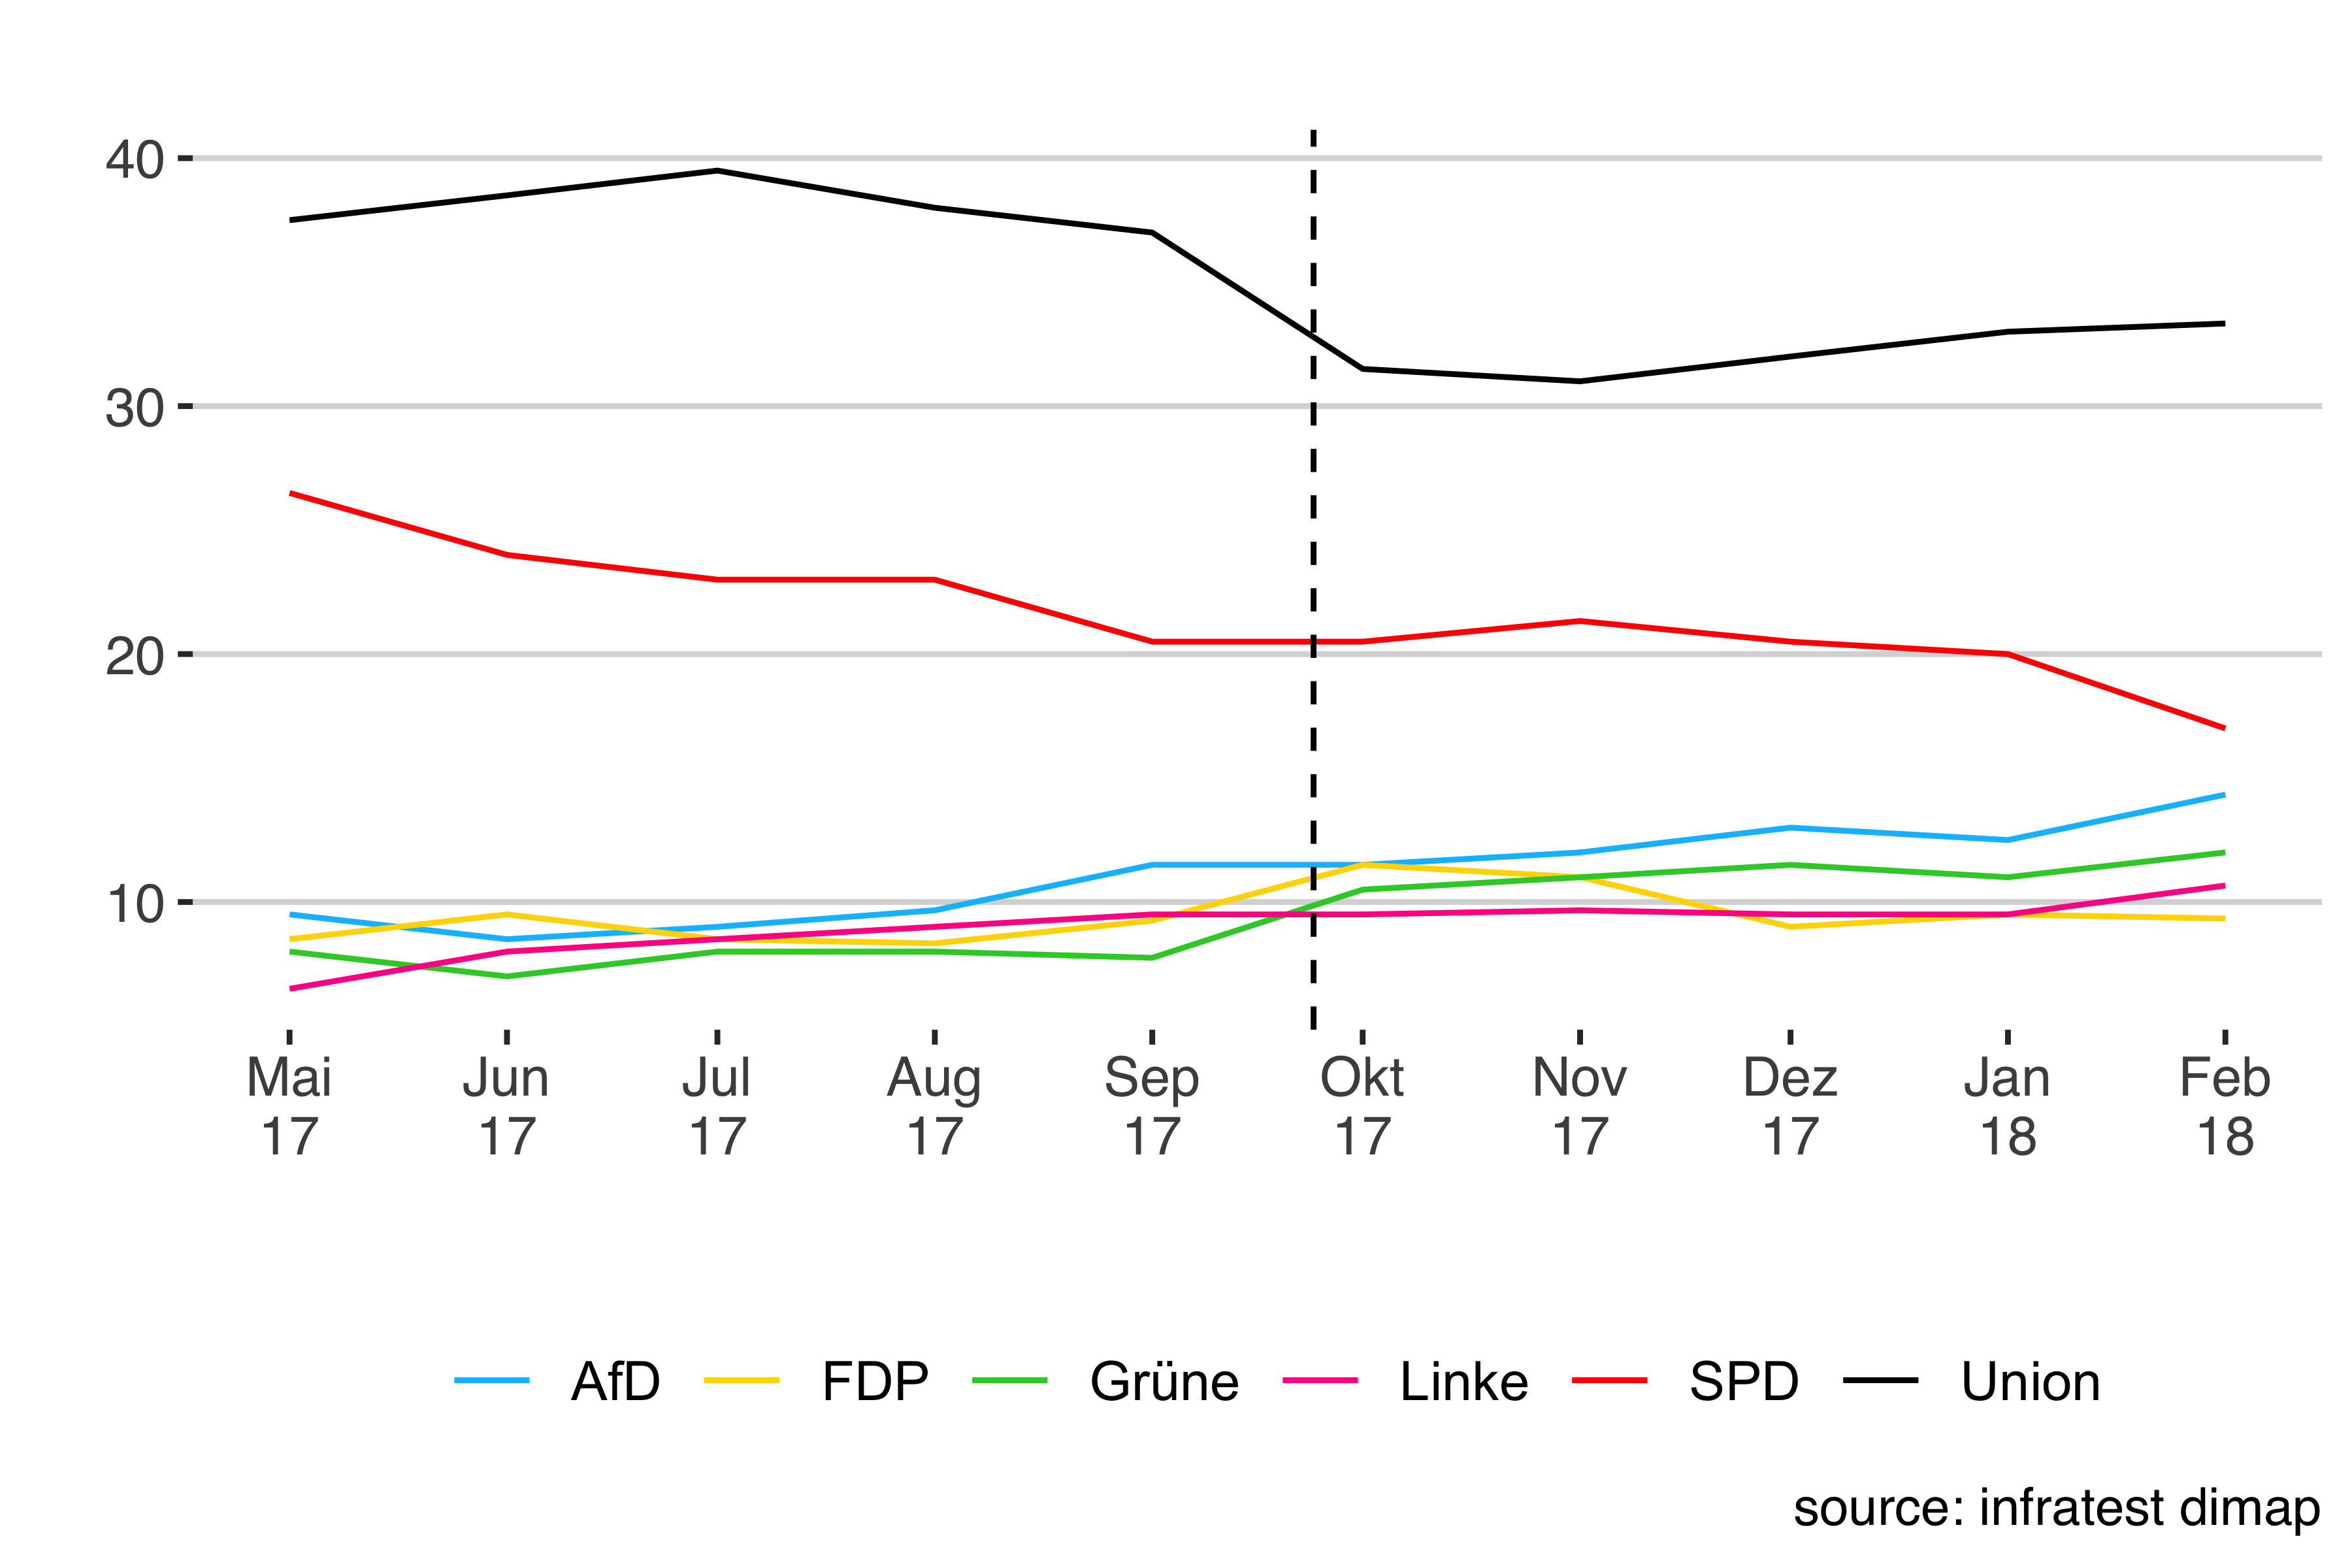
\includegraphics[width=0.8\textwidth]{figs/polls.png}
	\label{fig_polls}
	\end{center}
\end{figure}

% -----
% Data
% -----
\section{Dataset and data preparation}\label{ch_data}

%  An overview of the newspapers, including number of articles, online visits (as in  \citet{junque_de_fortuny_media_2012} )

% latex table generated in R 3.5.1 by xtable 1.8-3 package
% Sun Nov 11 21:36:13 2018
\begin{table}[ht]
\centering
\begin{tabular}{lrrr}
  \hline
medium & total\_articles & share & visits \\ 
  \hline
Bild.de & 3828 & 0.28 & 156867922 \\ 
  DIE WELT & 18663 & 0.14 & 52962285 \\ 
  FOCUS Online & 9235 & 0.22 & 68730873 \\ 
  SPIEGEL ONLINE & 5590 & 0.31 & 96139323 \\ 
  stern.de & 15804 & 0.15 & 18192672 \\ 
  tagesschau.de & 2261 & 0.41 & 75400000 \\ 
  ZEIT ONLINE & 5467 & 0.23 & 30600773 \\ 
   \hline
\end{tabular}
\caption{News sources used for the analysis} 
\end{table}


I conduct the estimation on a sample of 14,937 online news articles from seven German news providers about domestic politics\footnote{Bild.de, DIE WELT, FOCUS ONLINE, SPIEGEL ONLINE, stern.de, ZEIT ONLINE, Tagesschau.de}. The articles are dated from June 1, 2017 to March 1, 2018. I first extract all online articles using the Webhose.io API.\footnote{For more information see https://docs.webhose.io/v1.0/docs/getting-started. The scraping code was written in Python and can be made available on request.} Then all articles from the section "domestic policy" are filtered by using the URL of an article. Overall, the selected news providers are among the top ten German online news providers - in terms of unique user\footnote{The term unique user refers to a number of different visitors to a website within a certain period of time. Multiple visits from the same user are only considered once.} - in the period under review, with only Tagesschau.de belonging to the public media. The reason for this is that the content structure of Tagesschau.de is most similar to that of the private providers. ZDF.de offers predominantly video content and DLF (Deutschlandfunk) website mainly offers audio content in the form of interviews, which makes it hard to include it in the model. 

 Figure \ref{fig_distr1} shows the distribution of the number of articles by date. There is a high peak around the federal elections on September, 24th and another one shortly after the failure of the Jamaica coalition talks on November, 19th (indicated by the red dotted lines). Figure \ref{fig_distr2} shows that DIE WELT published the most articles on domestic policy, followed by stern.de and FOCUS ONLINE.  

\begin{figure}[H]
	\caption{Article distribution...}
	\begin{center}
		\begin{subfigure}[normla]{0.49\textwidth}
			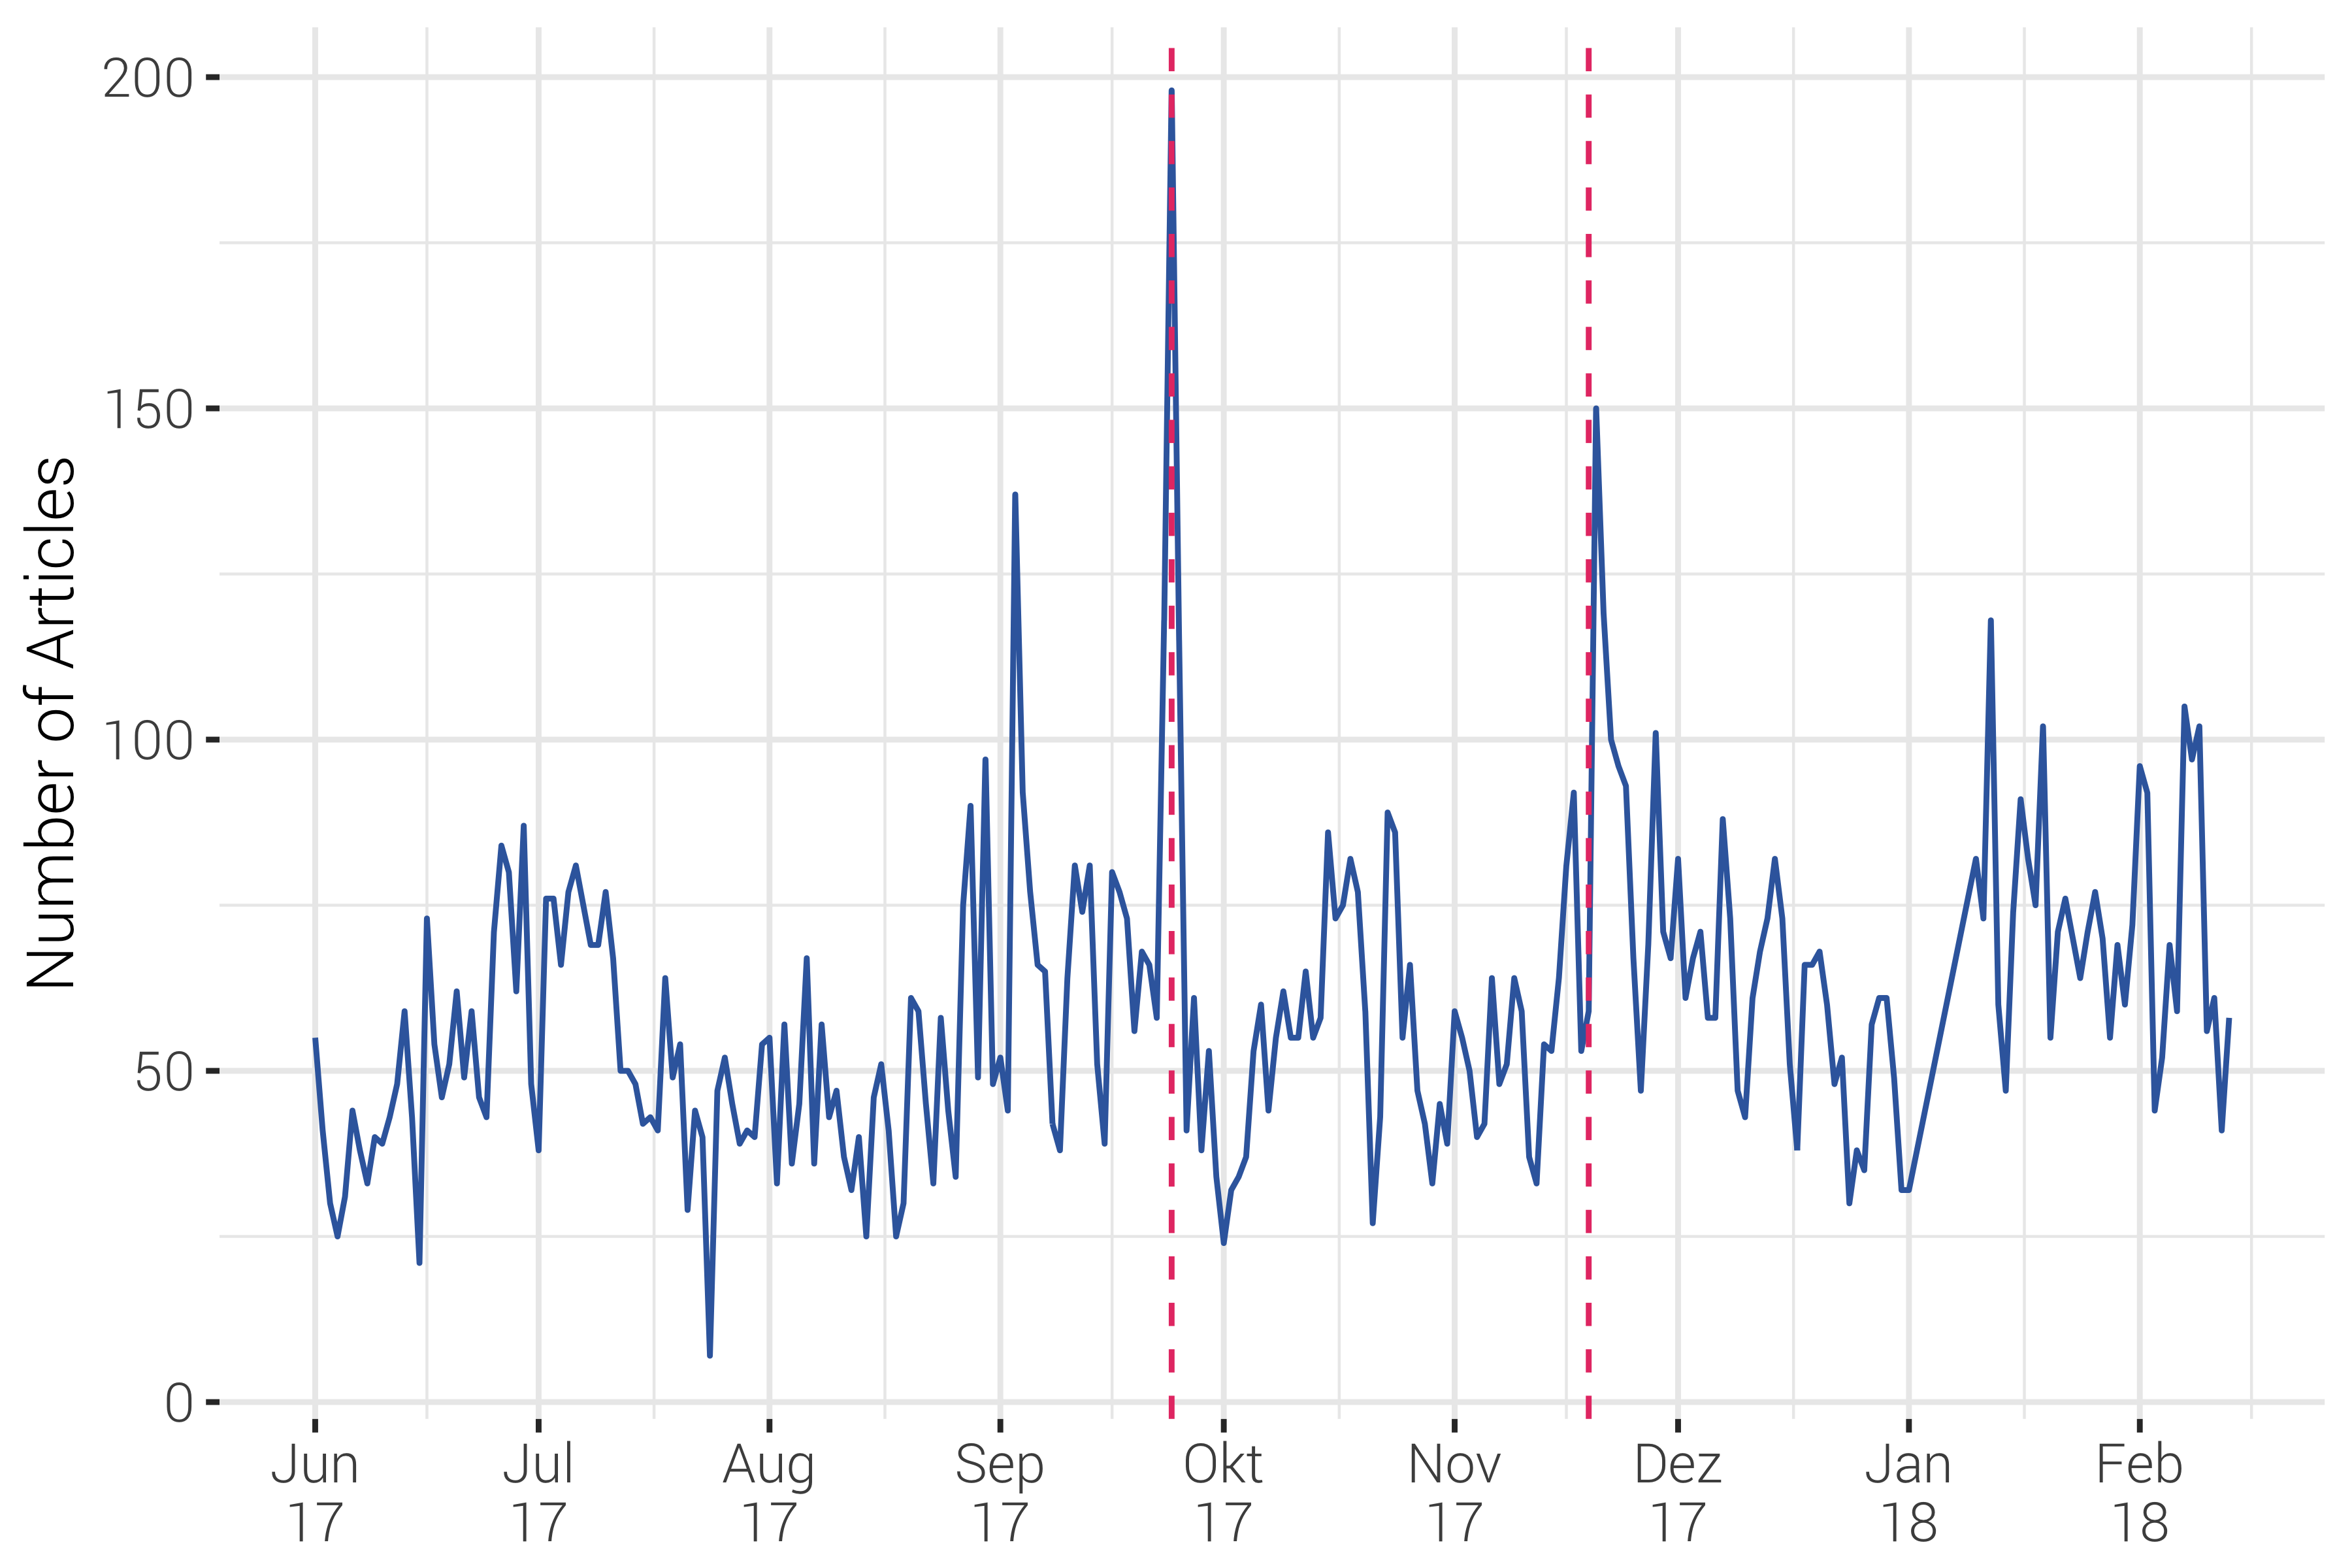
\includegraphics[width=\textwidth]{figs/timeline.png}
			\caption{...by date}
			\label{fig_distr1}
		\end{subfigure}
		\begin{subfigure}[normla]{0.49\textwidth}
			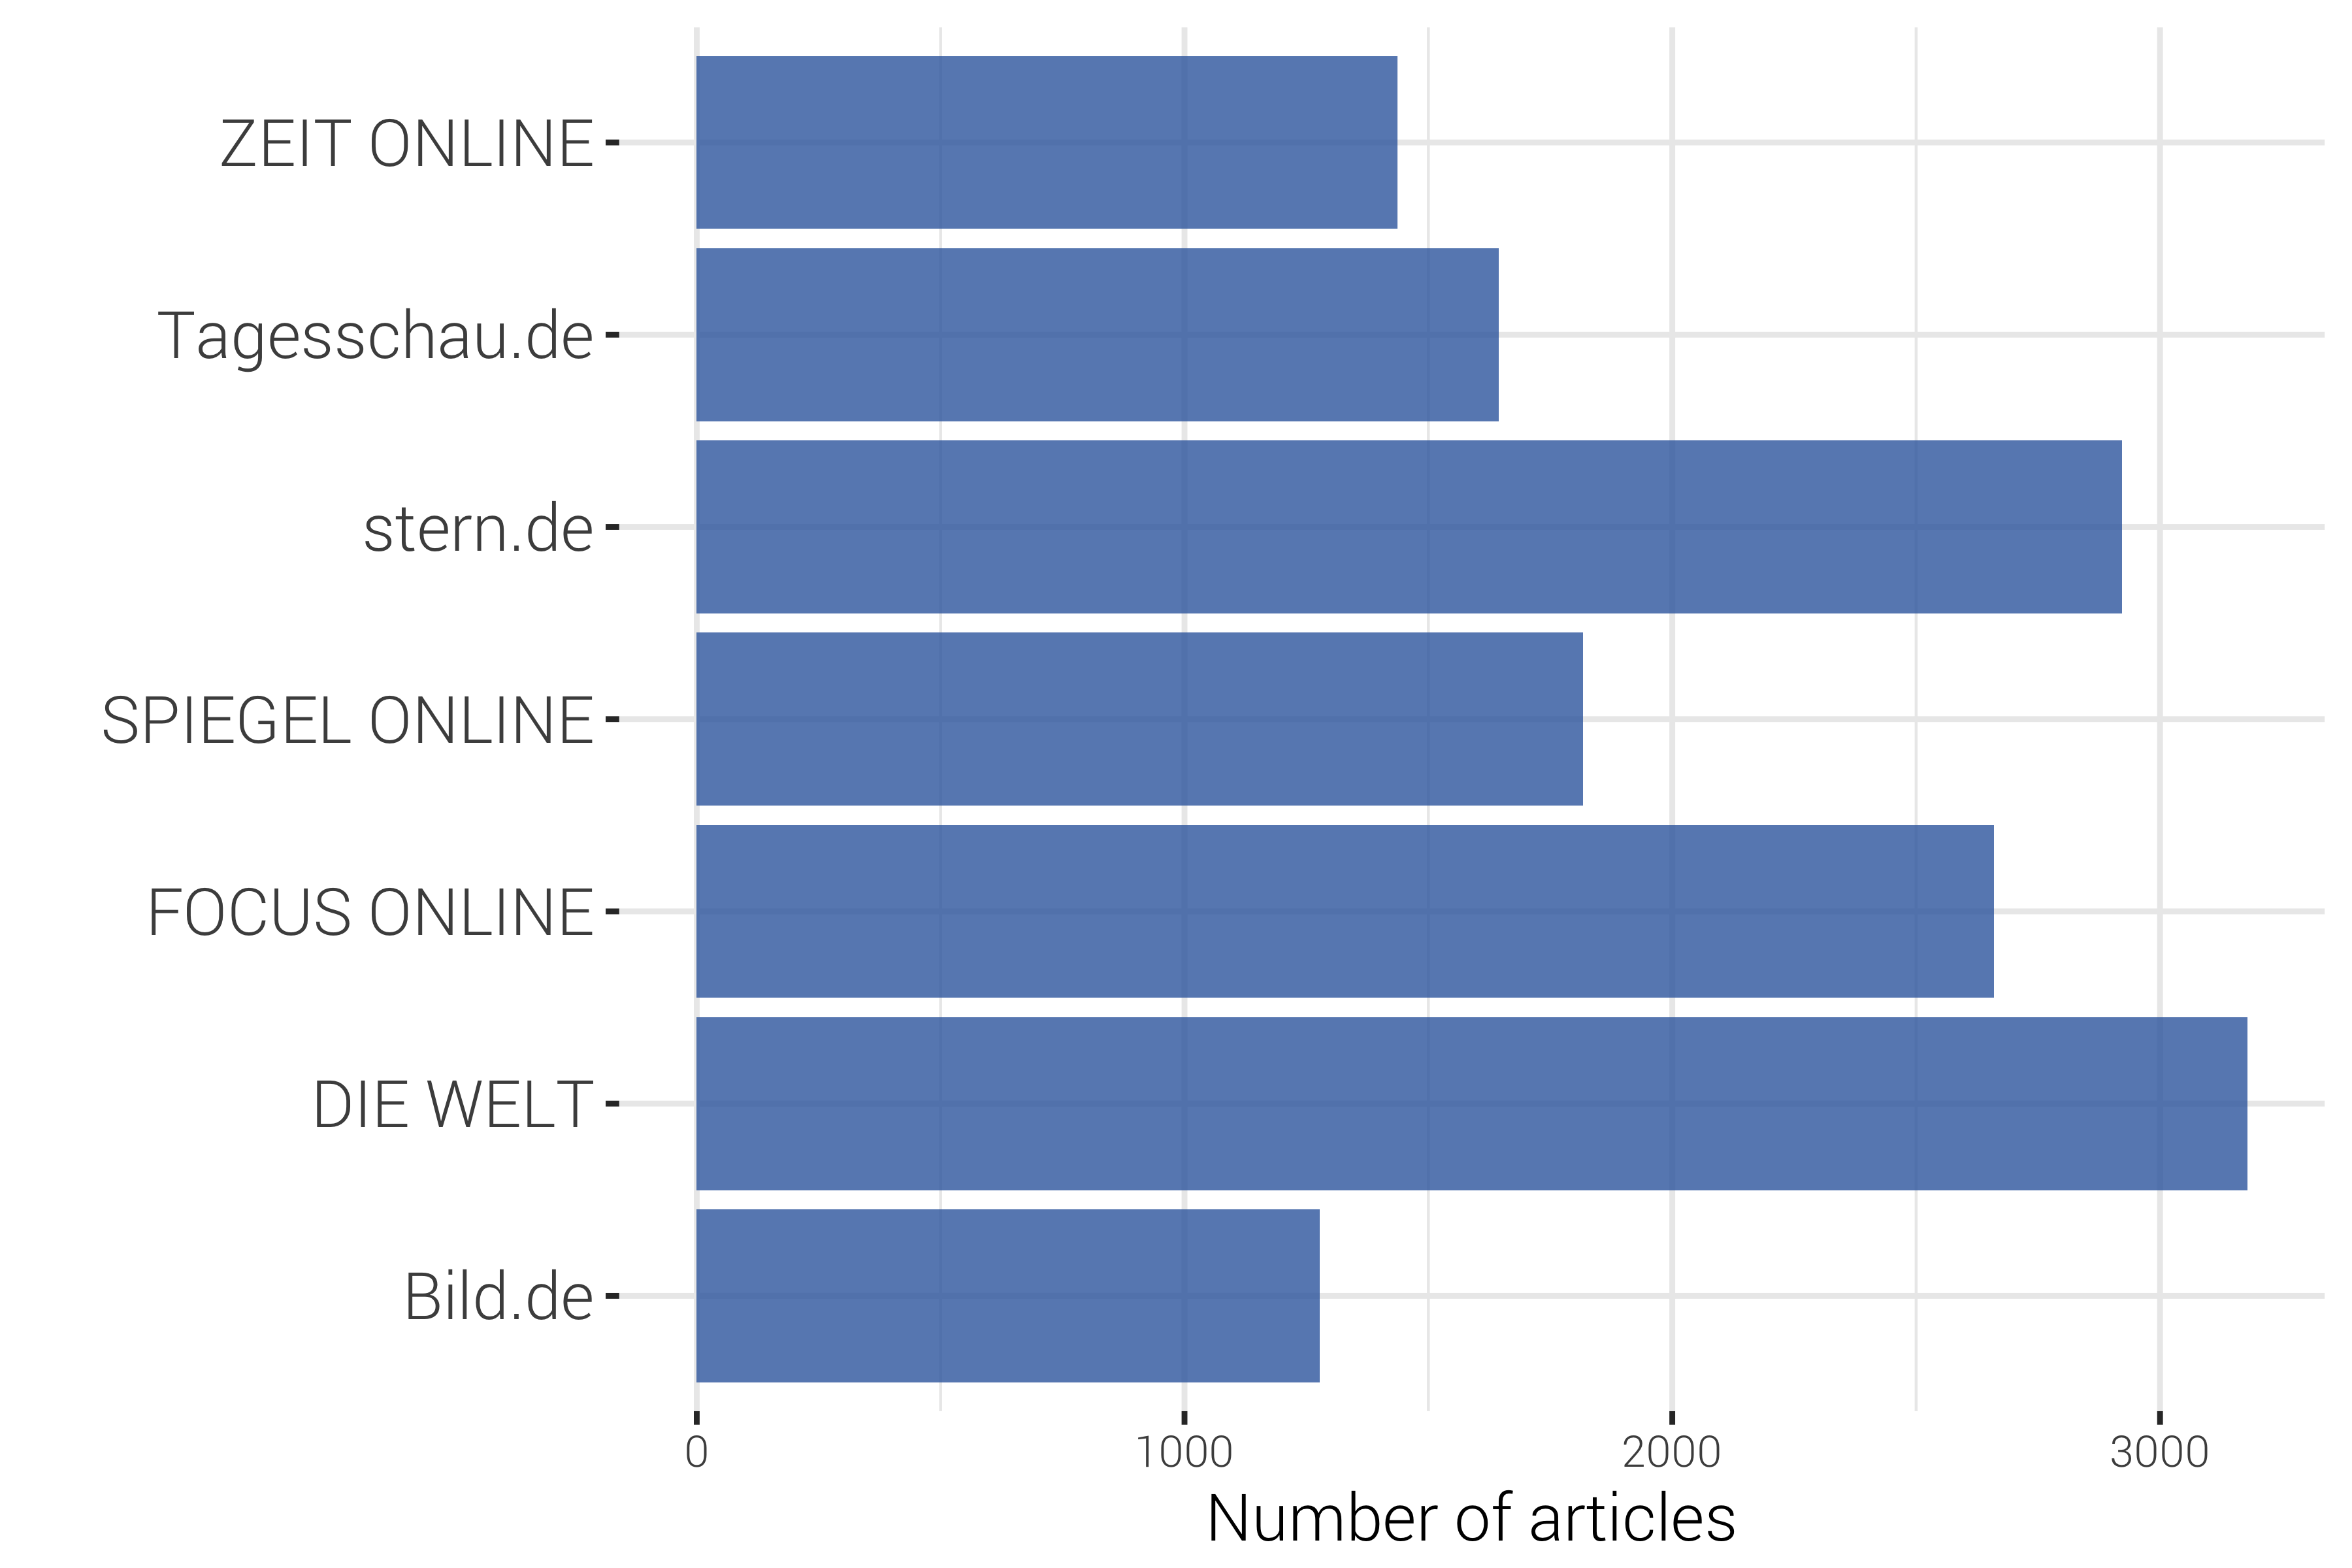
\includegraphics[width=\textwidth]{figs/bar.png}
			\caption{... by news provider}
			\label{fig_distr2}
		\end{subfigure}
	\end{center}
\end{figure}

Table \ref{t_textlength} gives an overview of the article length of the news pages. Most of the articles have a word length between 120 and 1000 words (articles with less than 121 words were filtered out in advance, as these were mostly reader comments). ZEIT ONLINE has the highest median (459 Words), followed by Tagessschau.de and Bild.de. 

% latex table generated in R 3.5.1 by xtable 1.8-2 package
% Sun Aug  5 20:19:16 2018
\begin{table}[ht]
\centering
\begin{tabular}{rlrrrrrrr}
  \hline
 & group1 & n & mean & sd & median & min & max & se \\ 
  \hline
1 & Bild.de & 1277.00 & 475.20 & 319.22 & 394.00 & 121.00 & 3710.00 & 8.93 \\ 
  2 & DIE WELT & 3179.00 & 507.88 & 614.28 & 377.00 & 121.00 & 14507.00 & 10.89 \\ 
  3 & FOCUS ONLINE & 2660.00 & 402.68 & 330.86 & 299.00 & 121.00 & 5647.00 & 6.42 \\ 
  4 & SPIEGEL ONLINE & 1817.00 & 498.96 & 333.23 & 387.00 & 121.00 & 3304.00 & 7.82 \\ 
  5 & Tagesschau.de & 1644.00 & 450.34 & 242.93 & 397.50 & 121.00 & 2006.00 & 5.99 \\ 
  6 & ZEIT ONLINE & 1437.00 & 510.98 & 377.85 & 459.00 & 121.00 & 8015.00 & 9.97 \\ 
  7 & stern.de & 2922.00 & 518.09 & 622.99 & 376.50 & 121.00 & 9287.00 & 11.53 \\ 
   \hline
\end{tabular}
\caption{Summary statistics of text length} 
\end{table}
\label{t_textlength}

To summarize the content of the texts, wordclouds help to get a first impression, as they represent the frequency of words by their size. Intuitively the term frequency (tf) of a word is a measure of how important that word may be for the understanding of the text. The word cloud in Figure \ref{fig_wordcloud1} is derived from all articles within the dataset. As can be seen, problems arise with words that are highly frequent. For example "die", or "der (eng. "the"), "und" (eng. "and"), and "ist" (eng. "is") are extremely common but unrelated to the quantity of interest. These terms, often called stop words \citep{gentzkow_text_2017}, are important to the grammatical structure of a text, but typically don't add any additional meaning and can therefore be neglected. A common strategy to reduce the number of language elements is to pre-process the text by imposing some preliminary restrictions (e.g. stop-word removal and stemming) based on the nature of the data (twitter text, newspaper articles, speeches, etc.) \citep{gentzkow_text_2017}. In fact, in order to use text as data and reduce the dimensionality to avoid unnecessary computational complexity and overfitting, pre-processsing the text is a central task in text mining \citep{bholat_text_2015}.  

\begin{figure}[H]
	\caption{Wordcloud (before pre-processing)}
	\begin{center}
		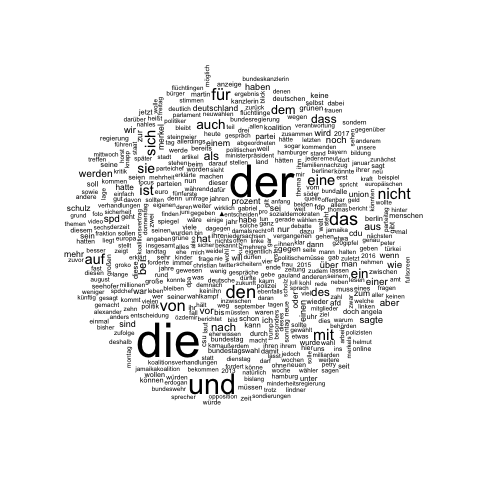
\includegraphics[width=0.7\textwidth]{figs/wordcloud.png}
		\label{fig_wordcloud1}
	\end{center}
\end{figure}

Stemming is a process by which different morphological variants of a word are traced back to their common root. For example, "voting" and "vote" would be treated as two instances of the same token after the stemming process. There are many different techniques for the stemming process. I apply the widely used Porter-Stemmer algorithm, which is based on a set of shortening rules that are applied to a word until it has a minimum number of syllables.\footnote{https://tartarus.org/martin/PorterStemmer/} To remove distorting words, the pre-defined stop word list from the Snowball project\footnote{http://snowball.tartarus.org/algorithms/german/stop.txt} is used together with a customized list of stop-words. Additionally punctuation character (e.g. ., ,, !, ?, etc.) and all numbers are removed from the data. After completing these steps we were left with 68,576 unique terms in our vocabulary. The following wordclouds represent the most frequent words of the pre-processed articles for Bild.de and Tagesschau.de.\footnote{The wordclouds of the other parties can be found in the appendix \ref{apx_wordclouds}} It becomes evident that these are texts discussing domestic policy issues. The SPD in particular seems to be highly frequent. However, at first glance, there are no obvious differences between the news providers.  

\begin{figure}[H]
	\caption{Wordclouds (after pre-processing)}
	\begin{center}
		\begin{subfigure}[normla]{0.48\textwidth}
			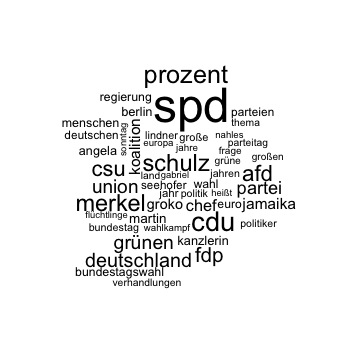
\includegraphics[width=\textwidth]{figs/wordcloud_Bild.png}
			\caption{Bild.de}
		\end{subfigure}
		\begin{subfigure}[normla]{0.48\textwidth}
			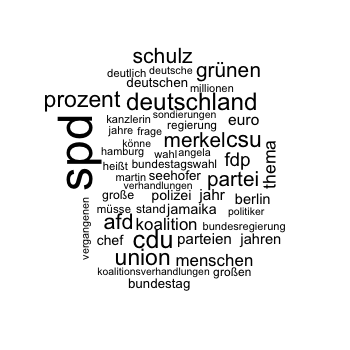
\includegraphics[width=\textwidth]{figs/wordcloud_Tagesschau.png}
			\caption{Tagesschau.de}
		\end{subfigure}
	\end{center}
\end{figure}

 % --------------------
% Document-term-matrix
% --------------------
To use text as data for statistical analysis, the next step is to divide the entire dataset into individual documents and to represent these documents as a finite list of unique terms. In this setting, each news article represents a document $d$, whereby each of these documents can be assigned to a news website. The sum of all documents forms what is called the corpus. For each document $d \in \lbrace 1,...,D \rbrace$ the number of occurrences of term $v$ in document $d$ is computed, in order to obtain the count $x_{d,v}$, where each unique term in the corpus is indexed by some $v \in \lbrace 1,...,V \rbrace$ and where $V$ is the number of unique terms. The $D$ x $V$ matrix $\boldsymbol{X}$ of all such counts is called the document-term matrix. Each row in this matrix represents a document, where each entry in this row counts the occurrences of a unique term in that document. This representation is often referred to as the bag of words model \citep{gentzkow_text_2017}, since the order in which words are used within a document is disregarded.
 

\section{Methodology}

Understand bias through its opposite (objectivity). In terms of news reporting this quality cirterion consists of many different aspects: (1) accuracy and realism, (2) separation of fact and opinion, (3) avoidance of slant (McQuail, 1992). 

In order to arrive at a better operational definition, some scholars argue that the opposite of bias is not necessarily objectivity but neutrality or balance \citep{hopmann_political_2012}. An unbiased news report is a neutral or balanced report, thus one that is not strongly slanted in favor of or against any political side. All sides should be equally represented according to some kind of benchmark for balance or neutrality. Conversely, in this view, bias is the extent to which media reporting deviates from this benchmark. The literature describes three types of media biases that may affect voters' party preferences: visibility bias, tonality bias, and agenda bias. In the next section, we describe each type of bias in turn and explain why each type is important for under- standing voter attitudes or behavior.



To ensure comparability between the bias metrics, they are standardized to range from −1 to 1, where a party would have a bias of 0 (neutral), when its visibility or tonality is equal to the mean visibility or tonality across all parties in that media outlet.

\subsection{Visibility Bias}

To determine visibility bias, we first need to measure visibility per se. We treat a party as visible in an article if the party itself is mentioned in an article. The overall visibility for each party is then defined by the relative amount of articles in which the party is present.
% Which benchmark ?
The next step is to define an appropriate reference point to distinguish between balanced/neutral and biased reporting. 
% list different approchase (D’Alessio & Allen, 2000, Hopmann et al. (2011b))
In another setting \citet{junque_de_fortuny_media_2012} uses the popularity in terms of votes as the a priori fair distribution. The visibility bias of a media source is the difference between the real distribution and the fair distribution.

To consider differences between parties as well as media outlets, the average visibility of all parties in each media outlet during the period of analysis is a key benchmark \citep{eberl_one_2017}. Our bias measure therefore captures whether party visibility is biased in comparison to what is typical for that outlet. Visibility bias is then computed as the deviation of each party’s specific visibility from the average visibility of all other parties in that outlet.

 

% ----------------------
% Structural topic Model
% ----------------------
\subsection{The structural topic model}\label{ch_model}

To find out the latent structure of each document, a structural topic model (STM) is estimated. In general, topic models formalize the idea that documents are formed by hidden variables (topics) that generate correlations among observed terms. They belong to the group of unsupervised generative models, meaning that the true attributes (topics) cannot be observed. One crucial assumption to be made for such models is the number of topics ($K$) that occur over the entire corpus. 

Each individual topic potentially contains all of the unique terms within the vocabulary $V$ with different probability. Therefore, each topic $k$ can be represented as a probability vector $\phi_k$ over all unique terms $V$. Simultaneously, each individual document $d$ in the corpus can be represented as a probability distribution $\theta_d$ over the $K$ topics. The underlying data generating process to generate each individual word $w_{d,n}$ in a document $d$ for the $n^{th}$ word-position can be described as follows:\footnote{A more detailed description of the generative process of the STM can be found in section \ref{ch_generativeProcess}}

\begin{enumerate}
	\item for each document $i$, draw its distribution of topics $\theta_d$ depending on the metadata included in the model; 
	\item for each topic $k$, draw its distribution of words $\phi_k$ depending on the metadata included in the model;
	\item for each word $n$, draw its topic $z_n$ based on $\theta_i$;
	\item for each word word $n$, draw the term distribution for the selected topic $\phi_{z_{d,n}}$.
\end{enumerate}

\todo{Assign a document to its highest probable topic?}
In section \ref{subsection_topic} the posterior distribution $\theta$ is used to estimate the conditional expectation of topic prevalence for given document characteristics. In order to calculate the sentiment value in section \ref{subsection_tone} each document $d$ is assigned to the topic with the highest probability ($\max (\theta_{k})$ for each document $d$).

The STM developed by \citet{roberts_model_2016} is a recent extension of the standard topic modelling technique, labeled as latent Dirichlet allocation (LDA), which refers to the Bayesian model in \citet{blei_latent_2003} that treats each word in a topic and each topic in a document as generated from a Dirichlet - distributed prior.\footnote{See also \citet{griffiths_probabilistic_2002}, \citet{griffiths_finding_2004} and \citet{hofmann_probabilistic_1999}. \citet{pritchard_inference_2000} introduced the same model in genetics for factorizing gene expression as a function of latent populations.} Since its introduction into text analysis, LDA has become hugely popular and especially useful in political science.\footnote{see \citet{blei_probabilistic_2012}, \citet{grimmer_text_2013} and \citet{wiedmann_text_2016} for an overview in social science and \citet{gentzkow_text_2017} give an overview of text mining applications in economics.} \citet{wiedmann_text_2016} uses topic model methods on large amounts of news articles from two german newspapers published between 1959 and 2011, to reveal how democratic demarcation was performed in Germany over the past six decades. \citet{paul_cross-collection_2009} compares editorial differences between media sources, using cross-collection latent Dirichlet allocation (ccLDA), an LDA-based approach that incorporates differences in document metadata. They use a dataset of 623 news articles from August 2008 from two American media outlets - msnbc.com and foxnews.com - to compare how they discuss topics. Reviewing the top words of the word-topic distribution, they find some content differences between the two media sources under review. 

The difference between the widely used LDA and the STM approaches lies in how $\theta$ and $\phi$ are determined. LDA assumes that $\theta ~ \text{Dirichlet}(\alpha)$ and $\phi ~ \text{Dirichlet}(\beta)$, where $\alpha$ and $\beta$ are fitted with the model. While for STM, the prior distributions for $\theta$ and $\phi$ depend on document-level covariates (e.g. the author or date of a document). For this purpose, the the STM specifies two design matrices of covariates, where each line defines a vector of covariates for a specific document.  In $X$, the covariates for topic prevalence are given, so that the probability of a topic for each document varies according to X, rather than resulting from a single common prior. The same applies to $Z$, in which the covariates for the word distribution within a topic are specified. 

The model has been applied to multiple academic fields: \citet{roberts_structural_2014} uses STM to analyze open-ended responses from surveys and experiments, \citet{farrell_corporate_2016} applies the model to scientific texts on climate change, revealing links between corporate funding and the framing of scientific studies. \citet{mishler_using_2015} show that "STM can be used to detect significant events such as the downing of Malaysia Air Flight 17" when applied to twitter data. Another study shows how STM can be used to explore the main international development topics of countries'€™ annual statements in the UN General Debate and examine the country-specific drivers of international development rhetoric \citep{baturo_what_2017}. \citet{mueller_reading_2016} use newspaper text to predict armed conflicts in different regions. They use the estimated topic shares in linear fixed effects regression to forecast conflict out-of-sample. \citet{roberts_navigating_2016} use STM to examine the role of partisanship in topical coverage using a corpus of 13,246 posts that were written for 6 political blogs during the course of the 2008 U.S. presidential election. With the aim of revealing the effect of partisan membership on topic prevalence, each blog is assigned to be either liberal or conservative. To explore the differences between the two, they look at the expected proportion of topics and examine the posts most associated with a respective topic. This approach is similar to \citet{roberts_model_2016}. 

% ----------------------
% Model Selection
% ----------------------
Inference of mixed-membership models, such as the one applied in this paper, has been a thread of research in applied statistics in the past few years (\citet{blei_latent_2003} \citet{erosheva_mixed-membership_2004} \citet{braun_variational_2010}). Topic models are usually imprecise as the function to be optimized has multiple modes, such that the model results can be sensitive to the starting values (e.g. the number of topics). Since an ex ante valuation of a model is hardly possible, I compute a variety of different models and compare their posterior probability. This enables me to check how results vary for different model solution \citep{roberts_navigating_2016}. I then cross-checked some subset of assigned topic distributions to evaluate whether the estimates align with the concept of interest \citep{gentzkow_text_2017}. These manual audits are applied together with numeric optimization based on the topic coherence measure suggested by \citet{mimno_optimizing_2011}. 

This process revealed that a model with 55 topics best reflects the structure in the corpus. Furthermore, the source (news website or party) of a document is used as covariate in the topic prevalence. In other words, the corresponding news website or party of an article or press release influences the probability distribution of topics for that document. Additionally I assume that the topical content differs between news articles and press releases. 

\subsection{Sentiment Analysis}

A dictionary-based method is then applied to measure the tone (or sentiment) of a document. The idea of a sentiment analysis is to determine the attitude of a writer toward the overall tonality of a document. To conduct such an analysis, a lists of words (dictionary) associated with a given emotion, such as negativity is pre-defined by the analyst. The document is then deconstructed into individual words and the frequencies of words contained in a given dictionary are calculated. 

Such lexical or "bag-of-words"€ approaches are widely presented in the finance literature to determine the effect of central banks' monetary policy communications on asset prices and real variables (\citet{nyman_news_2018} \citet{tetlock_giving_2007}, \citet{tetlock_more_2008}). \citet{hansen_shocking_2016} use a similar approach to measure "the two Ts" (Topic and tone). They explore the effects of FOMC (Federal Open Market Committee) statements on both market and real economic variables. To understand the latent topic of a statement, they apply LDA on a corpus of 142 FOMC decision statements split into sentences. They then measure how the central bank is talking about that topic, using a dictionary approach. To calculate their score, they subtract the negative words from the positive words und divide this by the number of total words of the statement. A similar score is used by \citet{nyman_news_2018}, who measure the effect of narratives and sentiment of financial market text-based data on developments in the financial system. They count the number of occurrences of excitement words and anxiety words and then scale these numbers by the total text size as measured by the number of characters.

The present paper uses a dictionary that lists words associated with positive and negative polarity weighted within the interval of $[-1; 1]$. SentimentWortschatz\footnote{SentiWS for short. available here: http://wortschatz.uni-leipzig.de/de/download}, is a publicly available German-language resource for sentiment analysis, opinion mining, etc.. The current version of SentiWS (v1.8b) contains 1,650 positive and 1,818 negative words, which sum up to 15,649 positive and 15,632 negative words including their inflections, respectively. Table \ref{t_sentdict} shows ten examples entries of the dictionary.

% latex table generated in R 3.4.2 by xtable 1.8-2 package
% Wed May  9 00:35:00 2018
\begin{table}[ht]
\centering
\begin{tabular}{rlr}
  \hline
 & word & value \\ 
  \hline
1 & brisant & -0.00 \\ 
  2 & makel & -0.18 \\ 
  3 & vergöttern & 0.00 \\ 
  4 & gediegen & 0.08 \\ 
  5 & mühe & -0.00 \\ 
  6 & untreue & -0.33 \\ 
  7 & unhöflich & -0.00 \\ 
  8 & erschweren & -0.49 \\ 
  9 & addieren & 0.00 \\ 
  10 & fehlleistung & -0.00 \\ 
   \hline
\end{tabular}
\caption{Sentiment Dictionary (Sample)} 
\label{t_sentdict}
\end{table}


The sentiment score for each document $d$ is calculated  based on the weighted polarity values for a word, defined on an interval between -1 and 1. The score is then calculated from the sum of the words in a document (which can be assigned to a word from the dictionary) divided by the total number of words in that document:
 
\begin{equation}
	\text{SentScore}_d = \frac{|\text{positive polarity score}_d| - |\text{negative polarity score}_d|}{|\text{TotalWords}_d|}
\end{equation}

% ----------------------
% Model Results
% ----------------------
\section{Empirical Evaluation}\label{ch_empirical}

This section summarizes the results of the STM. Subsequently "the two T's" (Topic and Tone) of the corpus are analyzed according to the following approaches: (1) The document-topic probability $\theta_{dk}$ is used to estimate the conditional expectation of topic prevalence for given document characteristics (section \ref{subsection_topic}). A set of topics is selected, that most distinctly discuss a particular party or a topic related to the federal elections. (2) Articles that are assigned to the selected topics with the highest probability are then used to conduct a dictionary-based sentiment analysis (section \ref{subsection_tone}). In order to check whether the sentiment values of certain topics are correlated with the results of voting preferences, the cross correlation function between these two concepts is calculated in \ref{ch_correlation}.

\subsection{Topic}\label{subsection_topic}

In order to get an initial overview of the results, Figure \ref{fig_expected_freq} displays the topics ordered by their expected frequency across the corpus. To assign a label to each topic, I looked at the most frequent words in that topic and the most representative articles \citep{roberts_model_2016}. 

It becomes apparent that topic 4 about the coalition talks between CDU/CSU and SPD - the "Grand coalition" or "GroKo" - is the topic with the highest expected frequency in the whole corpus, followed by the topic about the so-called Jamaica parties (CDU/CSU, FDP and B90/Die Grünen), which was the first alternative to be negotiated directly after the elections.  

\begin{figure}[H]
	\begin{center}
	\caption{Expected topic proportion}
		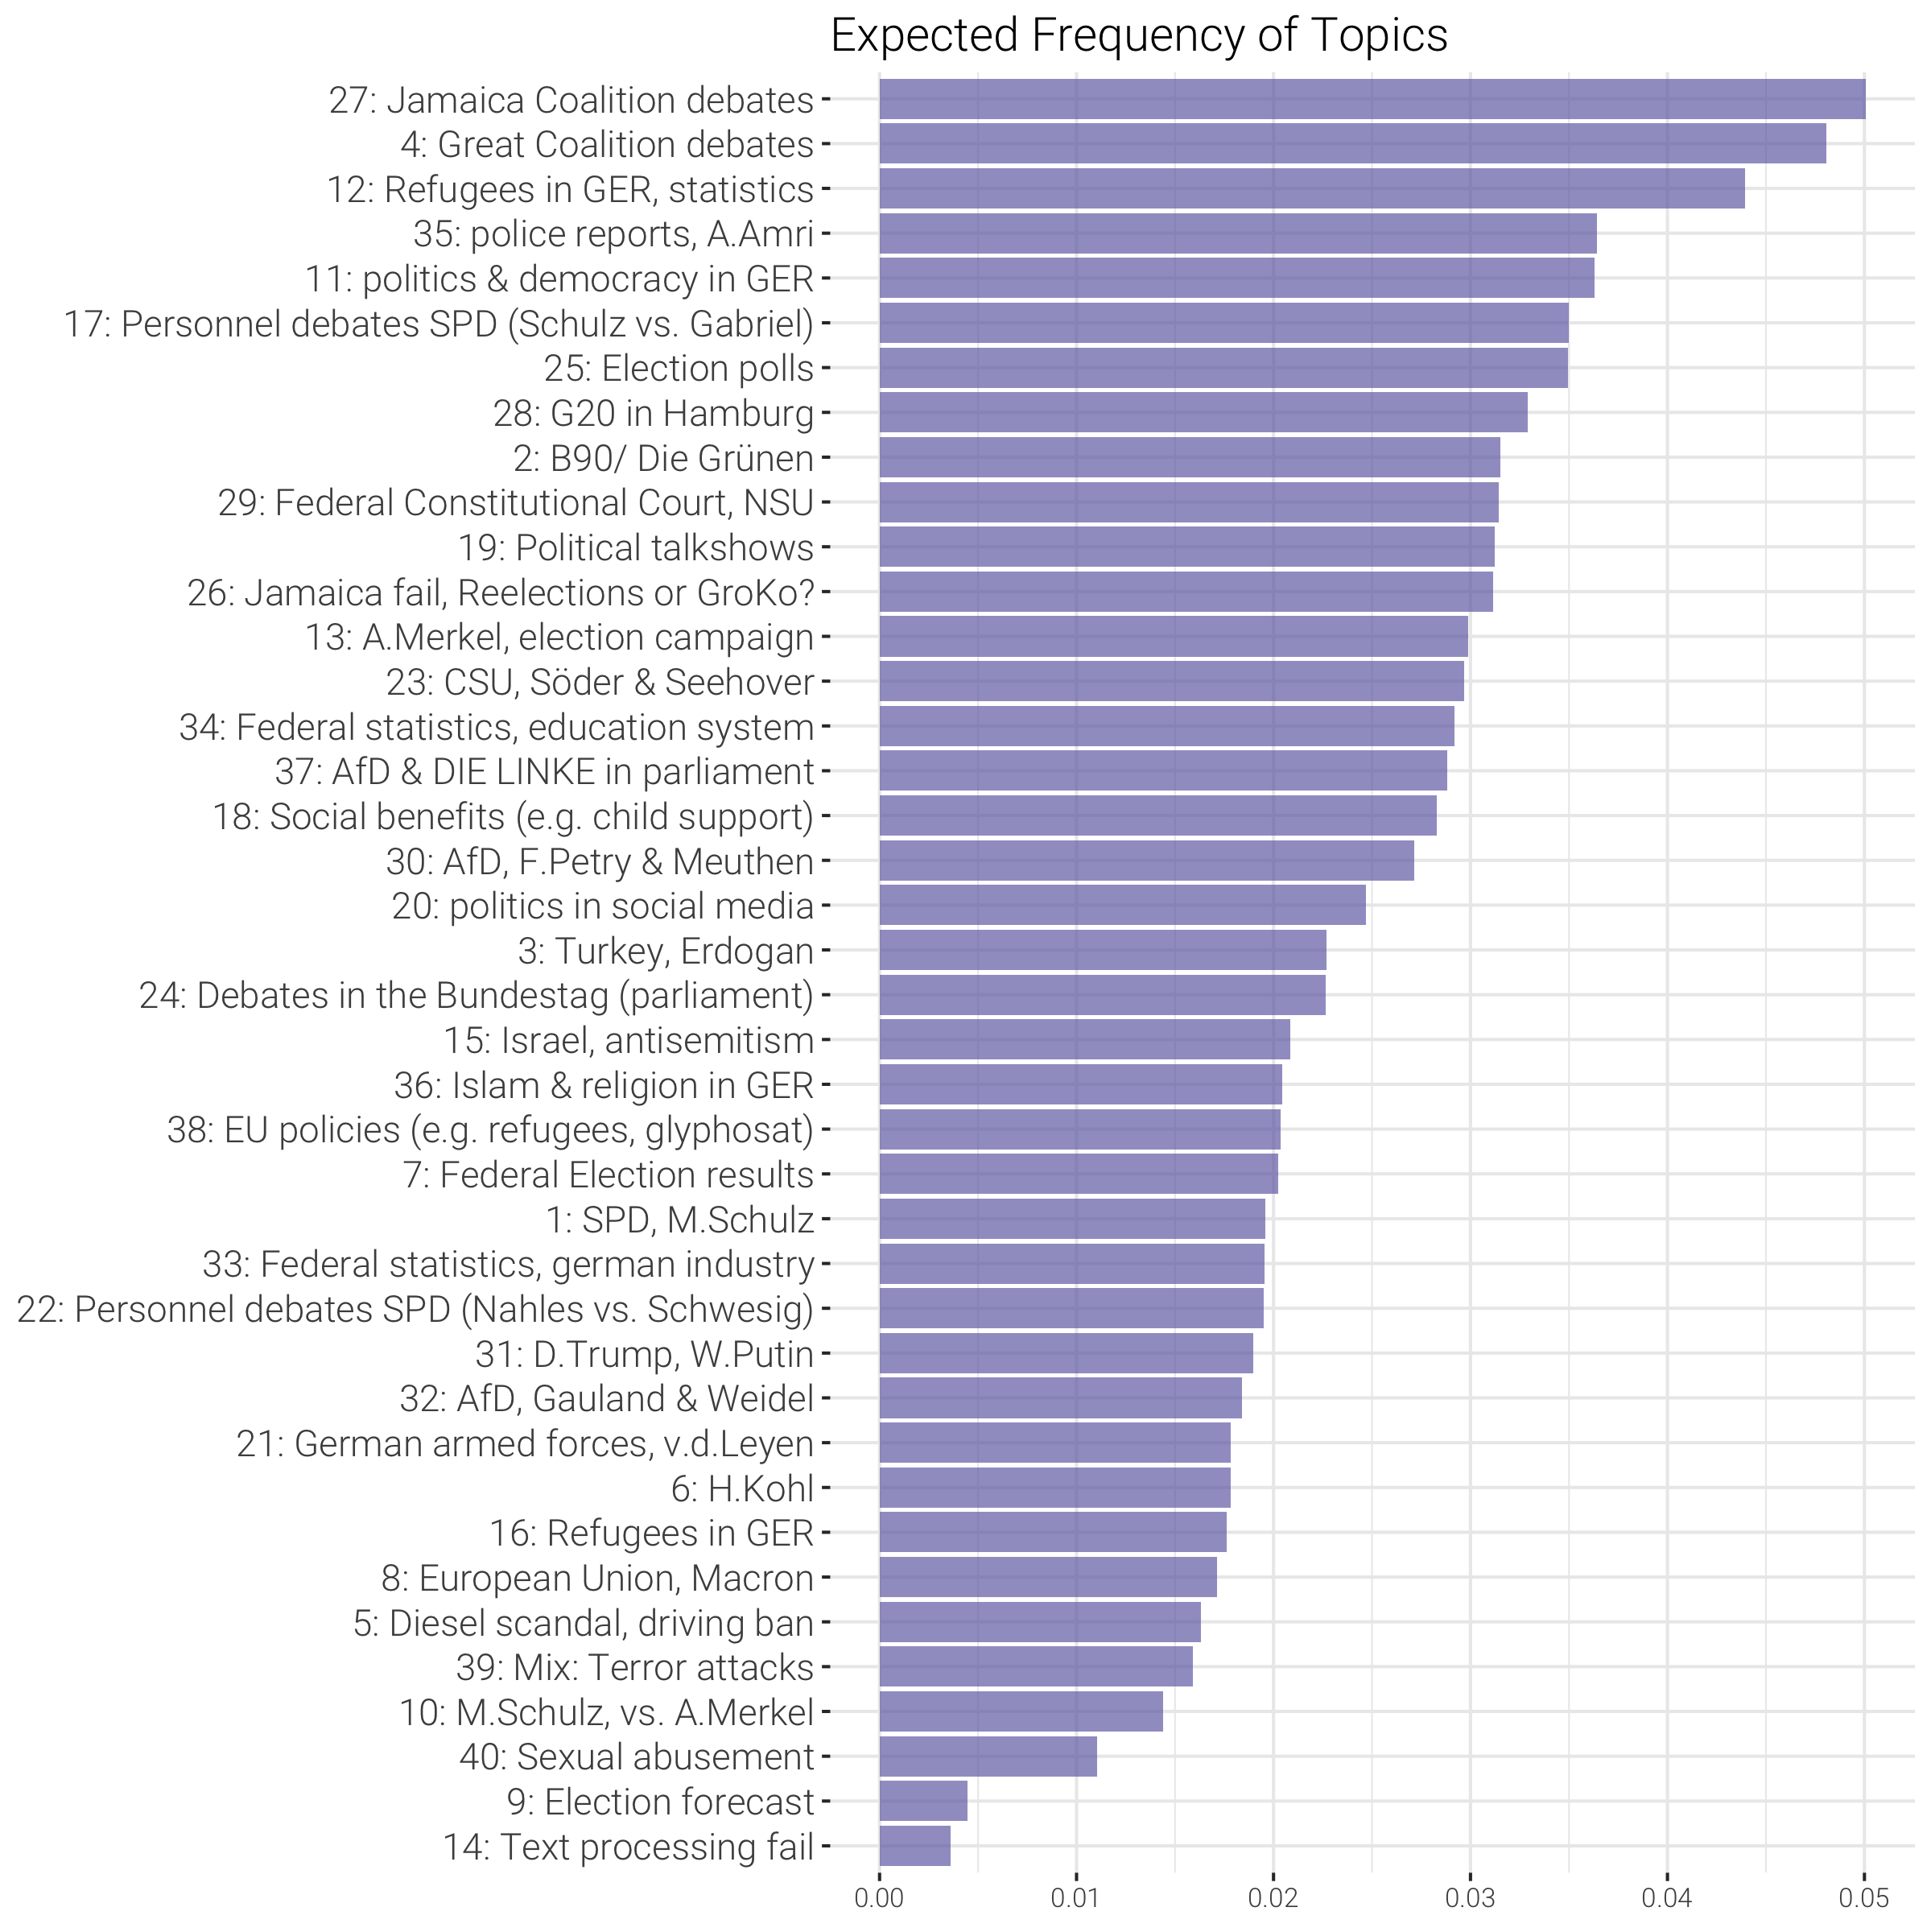
\includegraphics[width=\textwidth,keepaspectratio]{../figs/expected_freq.png}
		\label{fig_expected_freq}
\end{center}
\end{figure}

The remaining analysis is limited to topics closely related to one or more parties. For this reason, the following topics were selected. The most frequent words of these topics at each news website can be seen in Appendix \ref{apx_tf}: \todo{put this in the annex}

\begin{enumerate}
	\item Topic 1: About the SPD, mainly about the election campaign and Martin Schulz as candidate for the chancellor.	
	\item Topic 2: About B90/Die Grünen, mainly covering issues regarding the party's personnel debates.
	\item Topic 4: Covering the debates about the great coalition talks, mainly after the failure of the Jamaica coalition talks.
	\item Topic 13: About Angela Merkel, mainly about the election campaign. 
	\item Topic 17: Covering votes within the SPD, mainly regarding the vote about a possible coalition with CDU/CSU ("GroKo").	
	\item Topic 22: About SPD, mainly covering issues regarding the party's personnel debates
	\item Topic 23: About issues regarding the CSU, mainly about the competition between Horst Seehofer and Markus Söder and the negotiations with the CDU/CSU.
	\item Topic 26: Discussing the failure of the Jamaica coalition talks and the two possible alternatives: Reelections or a great coalition.
	\item Topic 27: Covering the Jamaica coalition talks, mainly focusing on the smaller players Bündnis B90/Die Grünen and FDP.	
	\item Topic 30: About the AfD, mainly about the resignation of Frauke Petry and Jörg Meuthen.
	\item Topic 32: About the AfD, mainly about Alice Weidel and Alexander Gauland, voted as parliamentary party leaders after the resignation of Frauke Petry.
	\item Topic 37: Covering debates of AfD and DIE LINKE in the parliament (Deutscher Bundestag).
\end{enumerate}   

To estimate the differences of topic prevalence of the mentioned topics for the different websites, a linear model is estimated for each topic $k$, where the documents are observations, the dependent variable is the posterior probability of the respective topic ($\theta_{d}$) and the covariates are dummy variables that are 1 if the document was published by the respective website and 0 otherwise (see equation \ref{eq_1}). To incorporate uncertainty in the dependent variable, a set of topic proportions are drawn from the variational posterior (the unnormalized topic proportions) repeatedly. Then, the coefficients are computed as the average over all results \citep{roberts_model_2016}.

\begin{equation}\label{eq_1}
\begin{split}
	\theta_{d}=\beta_0+\beta_1 x_{\text{FOCUS ONLINE,d}}+\beta_2 x_{\text{SPIEGEL ONLINE,d}}+\\
	\beta_3 x_{\text{stern.de,d}}+\beta_4 x_{\text{Tagesschau.de,d}}+\beta_5 x_{\text{DIE WELT,d}}+\\
	\beta_6 x_{\text{ZEIT ONLINE,d}}+\epsilon
\end{split}
\end{equation}

Figure \ref{fig_estimateEffects} shows the regression results for the topics selected above (see appendix \ref{apx_coeff} for the result tables). The coefficients indicate the deviation from the base value of Bild.de. Starting from above it becomes apparent that the topic prevalence of topic 46 (regarding the CDU/CSU) is significantly less for Tagesschau.de and Stern.de and significantly more for SPIEGEL ONLINE. The other media do not show any significant difference to Bild.de for this topic. The opposite is true for topic 37: With the exception of Stern.de and DIE WELT, topic prevalence for this topic is significantly higher for all media than for Bild.de. With the following two topics on AfD it is striking that the topic prevalence at Tagesschau.de is significantly lower compared to Bild.de. The topics concerning the Jamaican coalition (topic 27) and the failure (topic 26) seem to be discussed most likely at Bild.de. The case is different for the CSU issue (Topic 23), where SPIEGEL ONLINE has the highest probability. The same applies to the topic related to the personnel debates of the SPD (22). However, Bild.de has the highest topic prevalence for the topic related to votes within the SPD, especially the vote on the "GroKo" (17). The same applies to the topic regarding the SPD in general and Martin Schulz in particular (1). Overall, topics concerning the SPD seem to be more frequent at Bild.de than in the other media. Moreover, the distribution of topics at FOCUS ONLINE seems to be the most similar to that of Bild.de, while the biggest differences exist between Bild.de and Tagesschau.de. 

\begin{figure}[H]
	\caption{Regression results}
		\begin{center}
			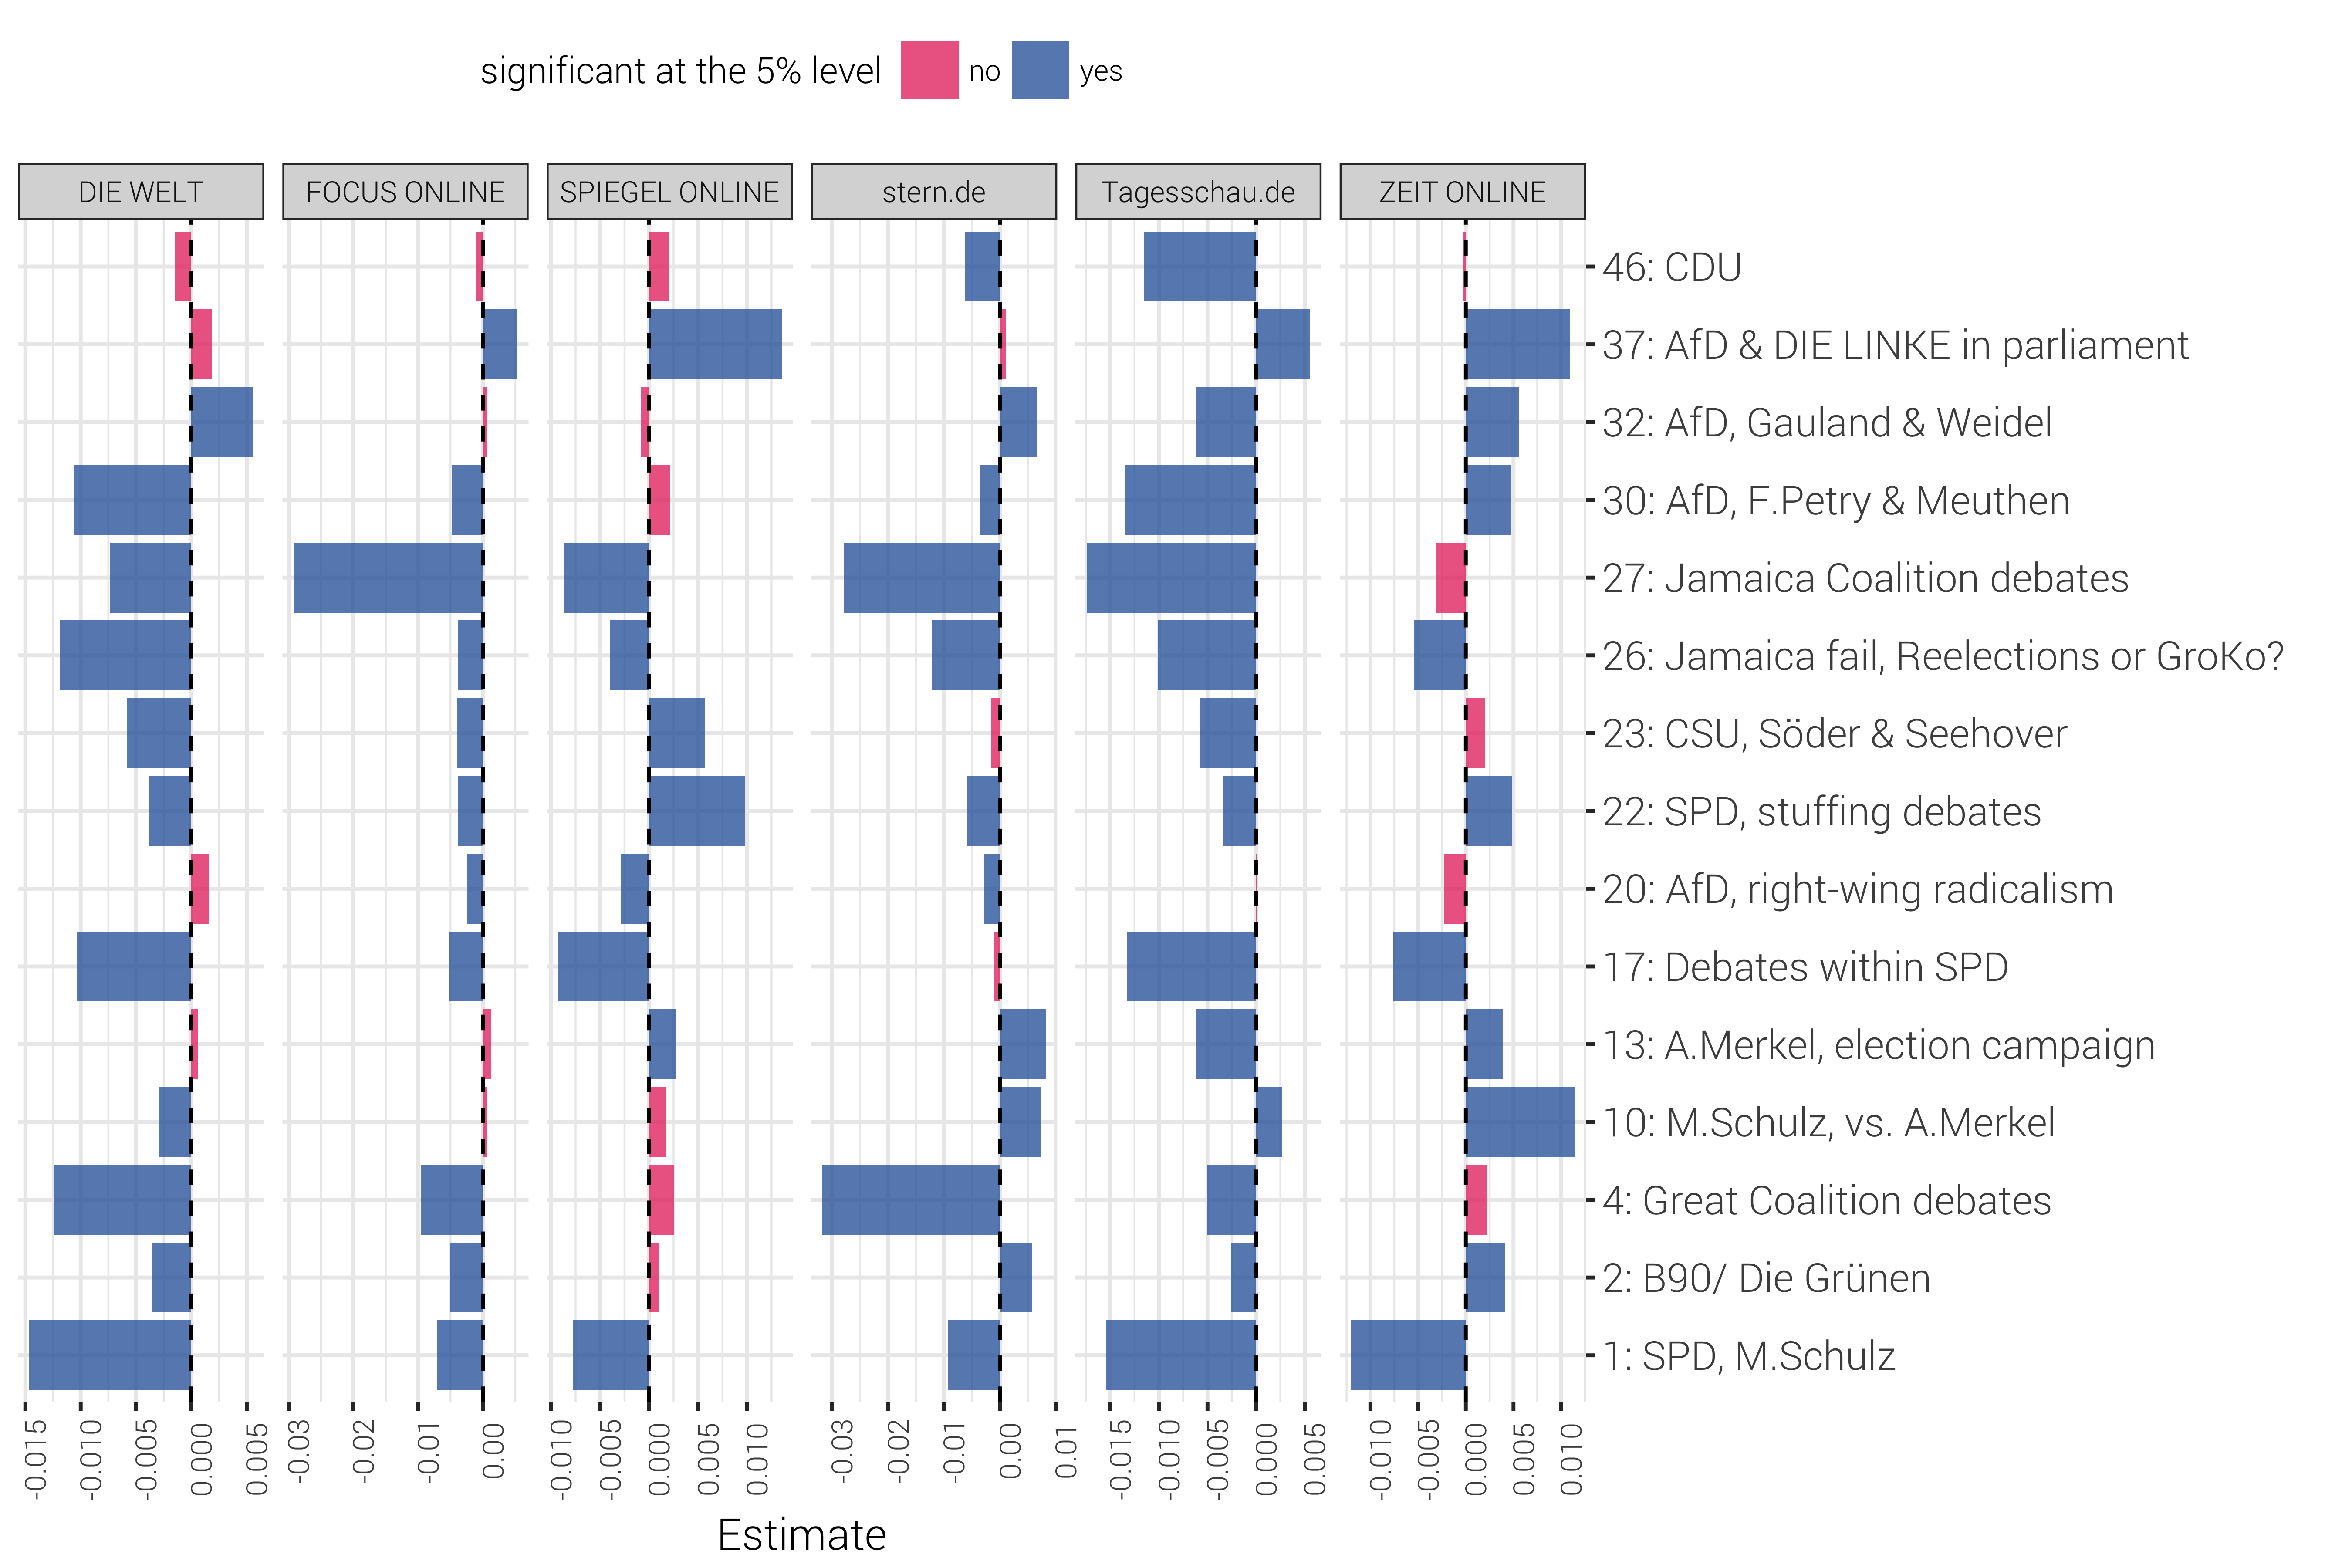
\includegraphics[width=\textwidth,keepaspectratio]{figs/estimates.png}
		\end{center}
	\label{fig_estimateEffects}
\end{figure}

% ---------------------------------%
% ------- Sentiment Analysis -------%

\subsection{Tone}\label{subsection_tone}

The results of the analysis for each topic on a monthly basis are listed in table \ref{apx_sentscore_monthly}, aggregated on all newspapers. Each sentiment value is weighted by the relative share of the topic in the overall reporting of that month. 

Some conclusions can be drawn from this table. First of all, it can be seen that, on monthly average, all topics are discussed almost exclusively negatively. An exception is topic 27 concerning the Jamaica coalition negotiations, which shows a positive sentiment value for a short period of time (October 2017).\footnote{Topics 22 and 26 also show positive values in July 2017, but the number of observations is very low.} 

Figure \ref{fig_sentscore_monthly} illustrates the values from the table normalized between 0 and 1. It becomes apparent that although topic 27 is the only one with a positive value, it also has the most negative value in the following month (November 2017), after it became clear that there would be no coalition between the CDU/CSU, FDP and Die Grünen. A similar trend can be observed for topic 26, which also includes the Jamaica Coalition: In November 2017, observations increase to 230 and the negative sentiment value rises sharply. Concerning the topic that discusses the great coalition between CDU/CSU and SPD (topic 4), it is evident that the overall tone in which this topic is discussed is generally decreasing from November 2017 to January 2018, but in the following February, the sentiment value of this topic rises. However, the sentiment score of topics that deal with the SPD (1, 17, 22) is diminishing in the course of time, with topic 17 recording the largest decline. For the other parties the process is rather zigzag-like. The figures shows no evidence for the reproach, that the mass media reports more negatively about the AfD.

\begin{figure}[H]
	\caption{Monthly Sentiment Score}
		\begin{center}
			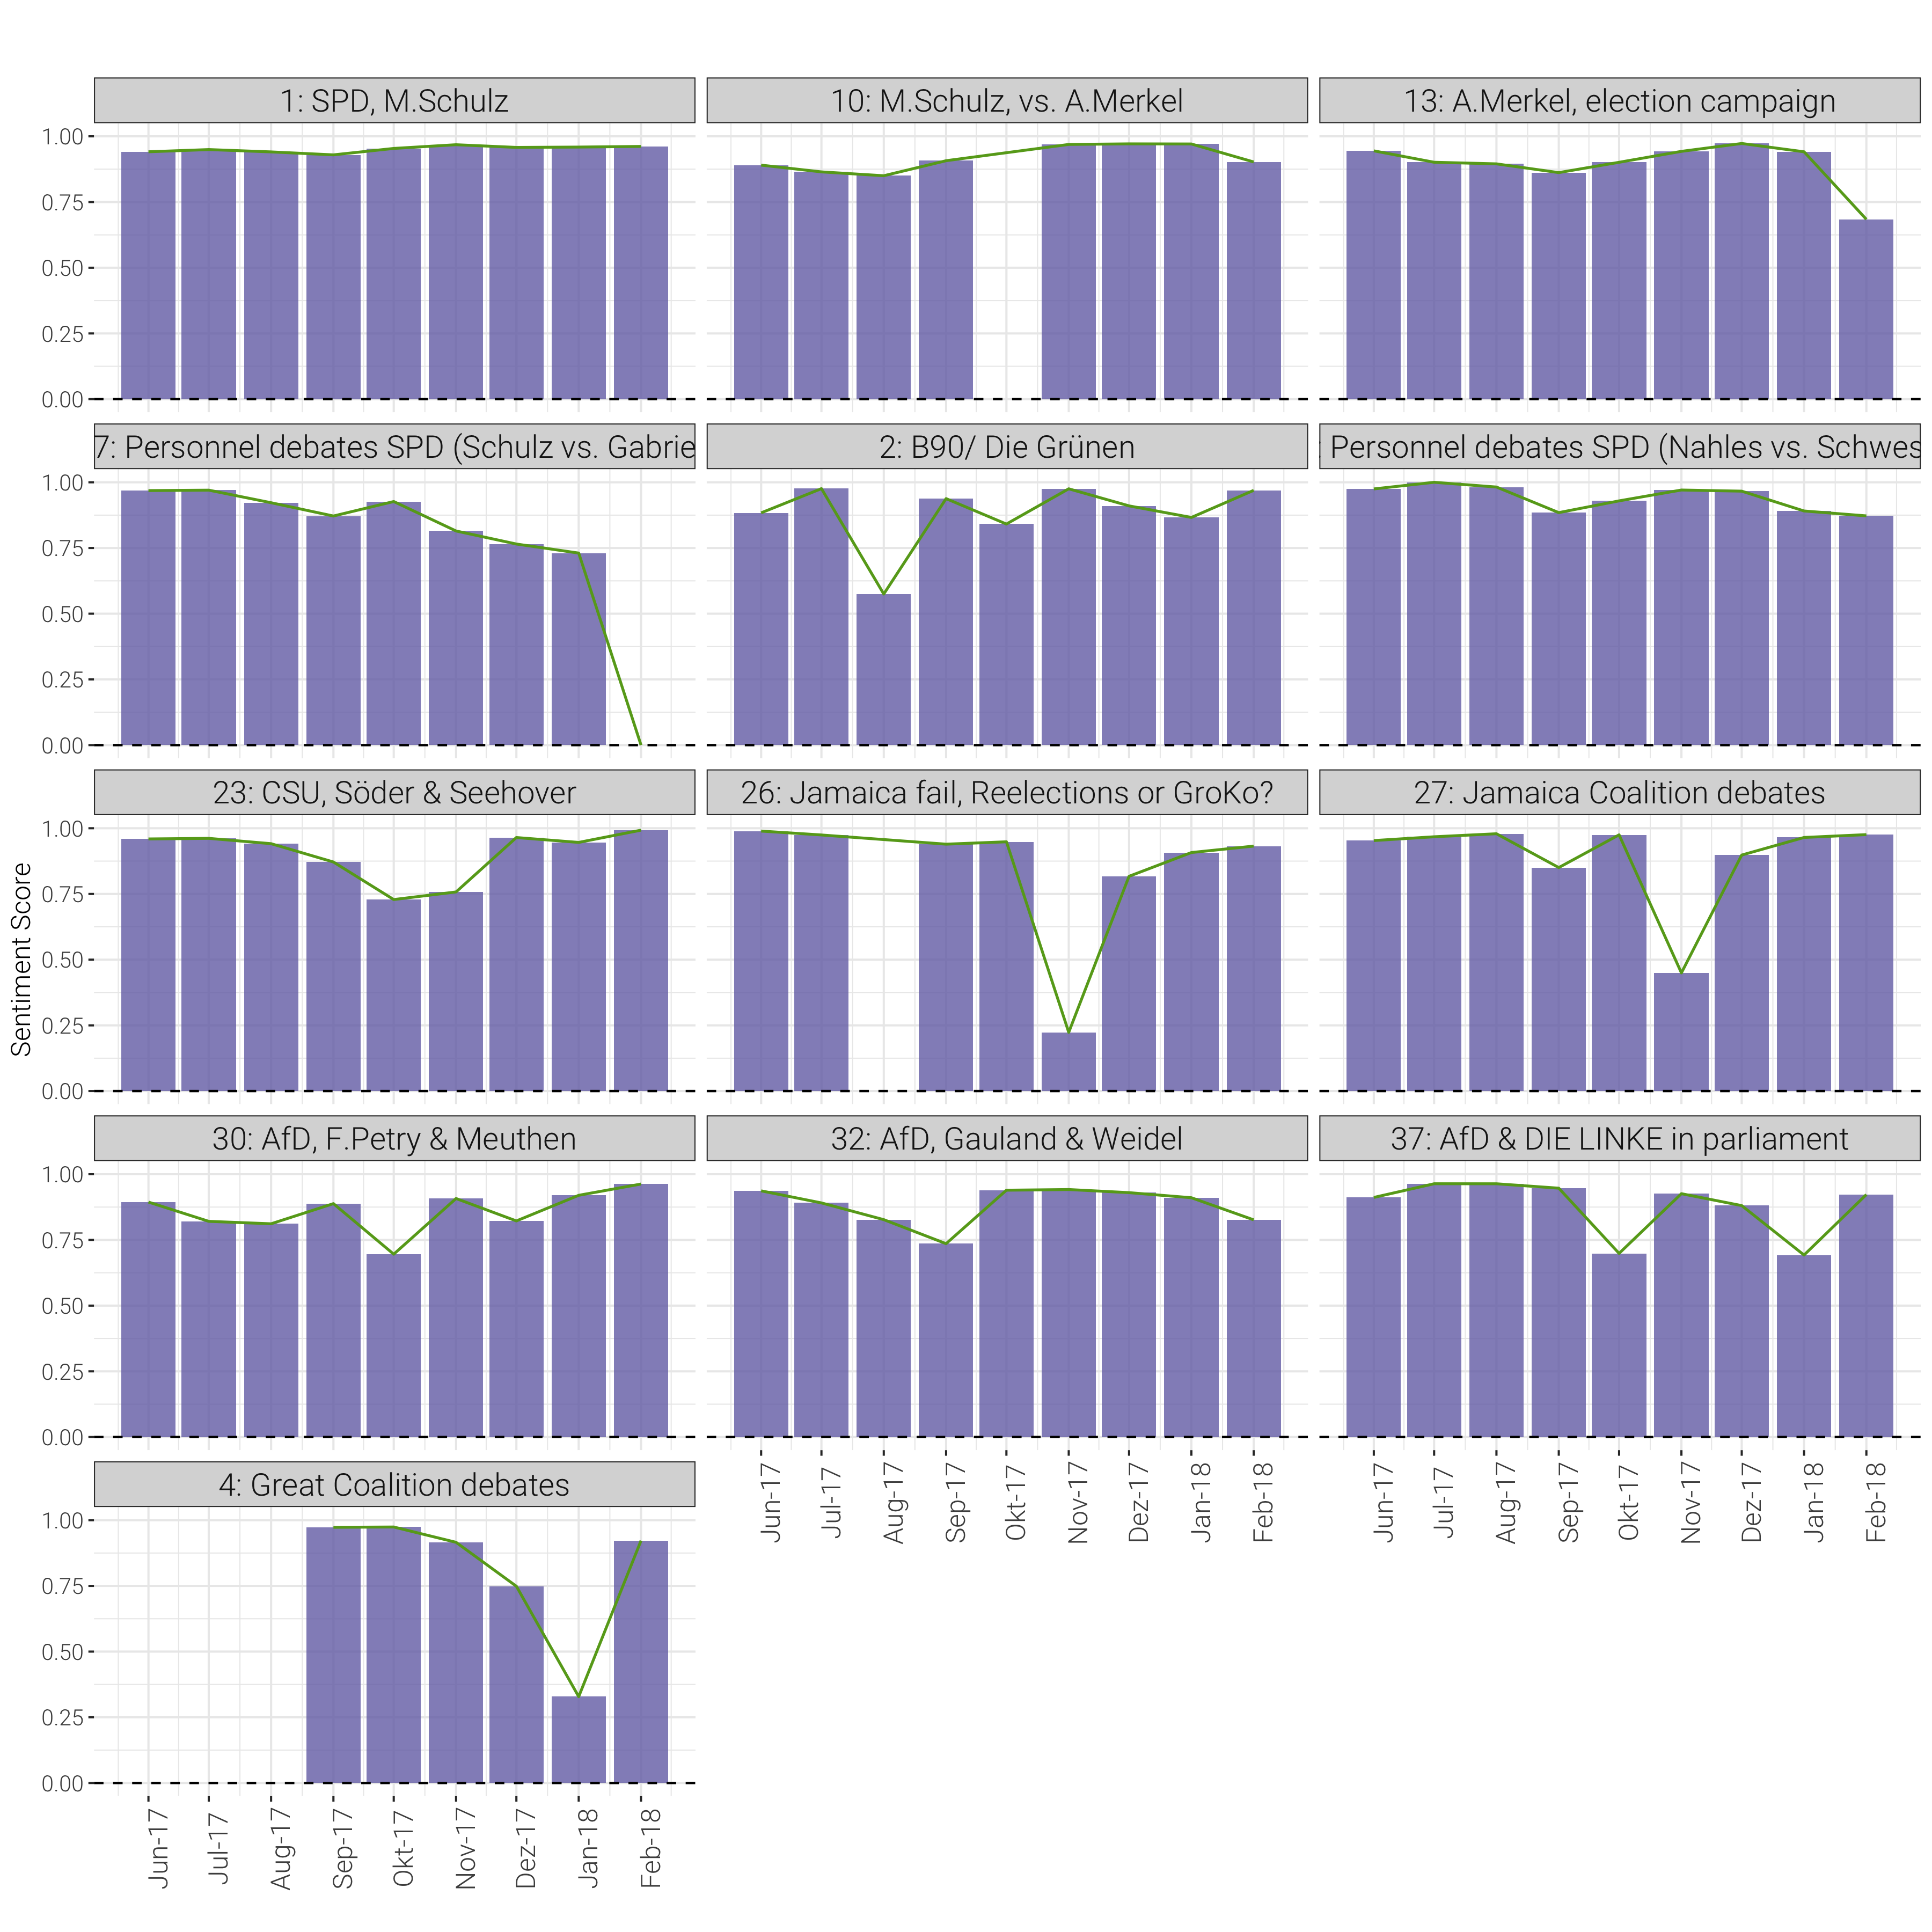
\includegraphics[width=0.9\textwidth,keepaspectratio]{figs/sentscore_monthly.png}
		\end{center}
	\label{fig_sentscore_monthly}
\end{figure}

The sentiment value aggregated by news provider is listed in table \ref{apx_sentscore_site}. Again, it becomes apparent, that all topics show a negative value. In order to analyze the differences between the news websites, two different figures are considered: (1) The bar plot is used to examine the polarity tendencies of the individual topics for a the respective website (Figure \ref{fig_sentscore_site}) and (2) the radar plot is considered to observe the differences between the websites (Figure \ref{fig_sentscore_radar}).

Starting with the bar plot it becomes apparent that  topics that include the coalition negotiations (26, 27, 4) and the SPD (1, 17) are the most negative at Bild.de. The topics relating to AfD (20, 30, 32, 37) are also discussed more negatively. Looking at the values of DIE WELT, two of the AfD topics have the most negative values (32, 20). Topic 27 concerning the Jamaica Coalition and the Grand Coalition (4) also score relatively negatively. Concerning FOCUS ONLINE, it is mainly topics that relate to the SPD (27, 17, 4, 1) that have a strong negative sentiment value, together with topic 32 and 37 - both related to AfD. Turning to SPIEGEL ONLINE, it is noticeable that the difference in sentiment value between the individual topics is less pronounced. Topics 13 (election campaign of A.Merkel) and 10 (A.Merkel vs M.Schulz) stand out as comparatively less negative. However, these issues are also the least negatively discussed in the other media. Also at stern.de the difference in sentiment value is less significant and overall less negative. The topics regarding CDU/CSU (46) and Martin Schulz (10) score the most positively (or least negatively). Tagesschau.de is the least negative on most topics, or even once positive. However, this does not apply to topic 23 (CSU), where tagesschau.de is most negative in comparison to the other media. As with Bild.de, the issues relating to the coalition negotiations (27 and 4) also come off rather badly with ZEIT ONLINE. However, the issues surrounding AfD (30, 32, 37 and 20) are even more negative than at Bild.de. 

\begin{figure}[H]
	\caption{Sentiment Score by news website}
	\begin{center}
			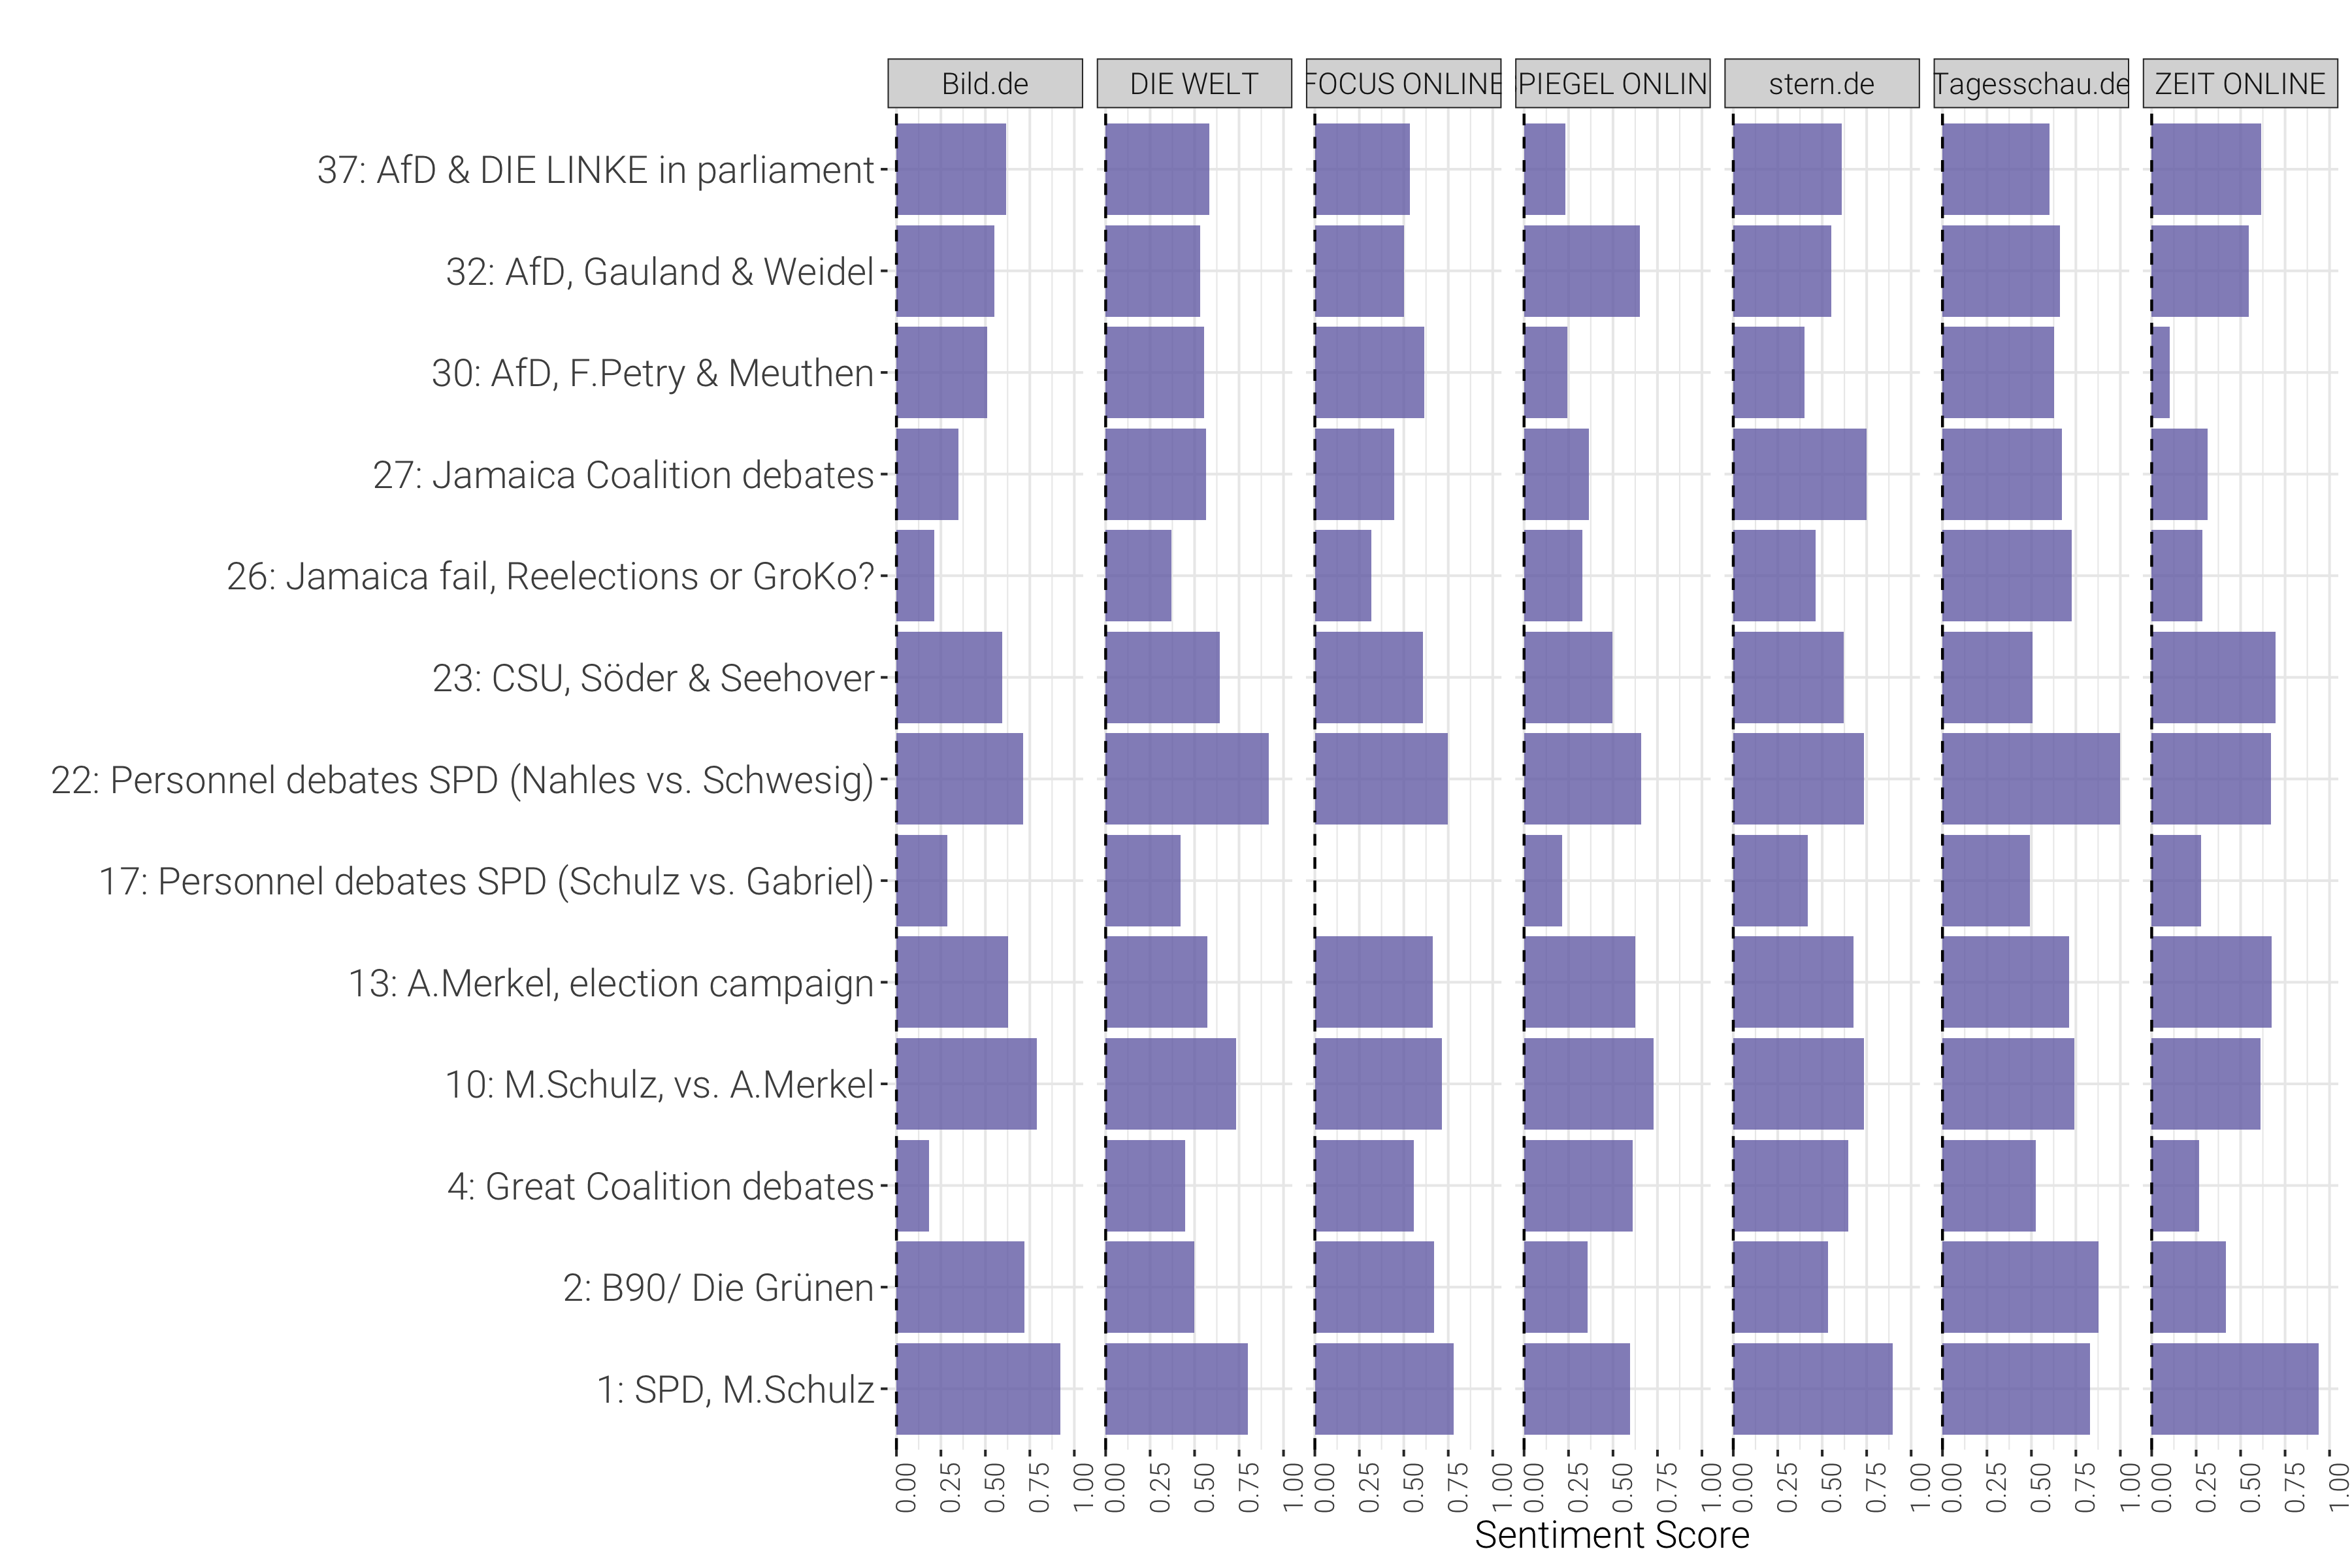
\includegraphics[width=\textwidth,keepaspectratio]{figs/sentscore_site.png}
			\label{fig_sentscore_site}
	\end{center}
\end{figure}

A good overview of how differently the topics are discussed by the providers is shown in Figure \ref{fig_sentscore_radar}. It becomes evident that the sentiment value of the media differs most notably with regard to topic 27 and topic 4, i.e. the topics on which the coalition negotiations are reported. With regard to the Jamaica coalition, Bild.de reports the most and tagesschau.de the least negative. The reporting of ZEIT ONLINE concerning the grand coalition is the one with the most negative sentiment value and again Tagesschau.de, together with stern.de, the one with the value which is least negative. Furthermore, it becomes evident that the negative sentiment value of FOCUS ONLINE regarding topic 17 is high in relation to the other media. FOCUS ONLINE thus reports comparatively more negatively on the debates within the SPD. This includes in particular the vote on a possible coalition with CDU/CSU/CSU. For topic 1, which also deals with the SPD, the value of FOCUS ONLINE is rather negative, only undercut by Bild.de. Topics related to AfD do not show striking differences. 

\begin{figure}[H]
	\caption{Radar Plot of Sentiment Scores}
	\begin{center}
			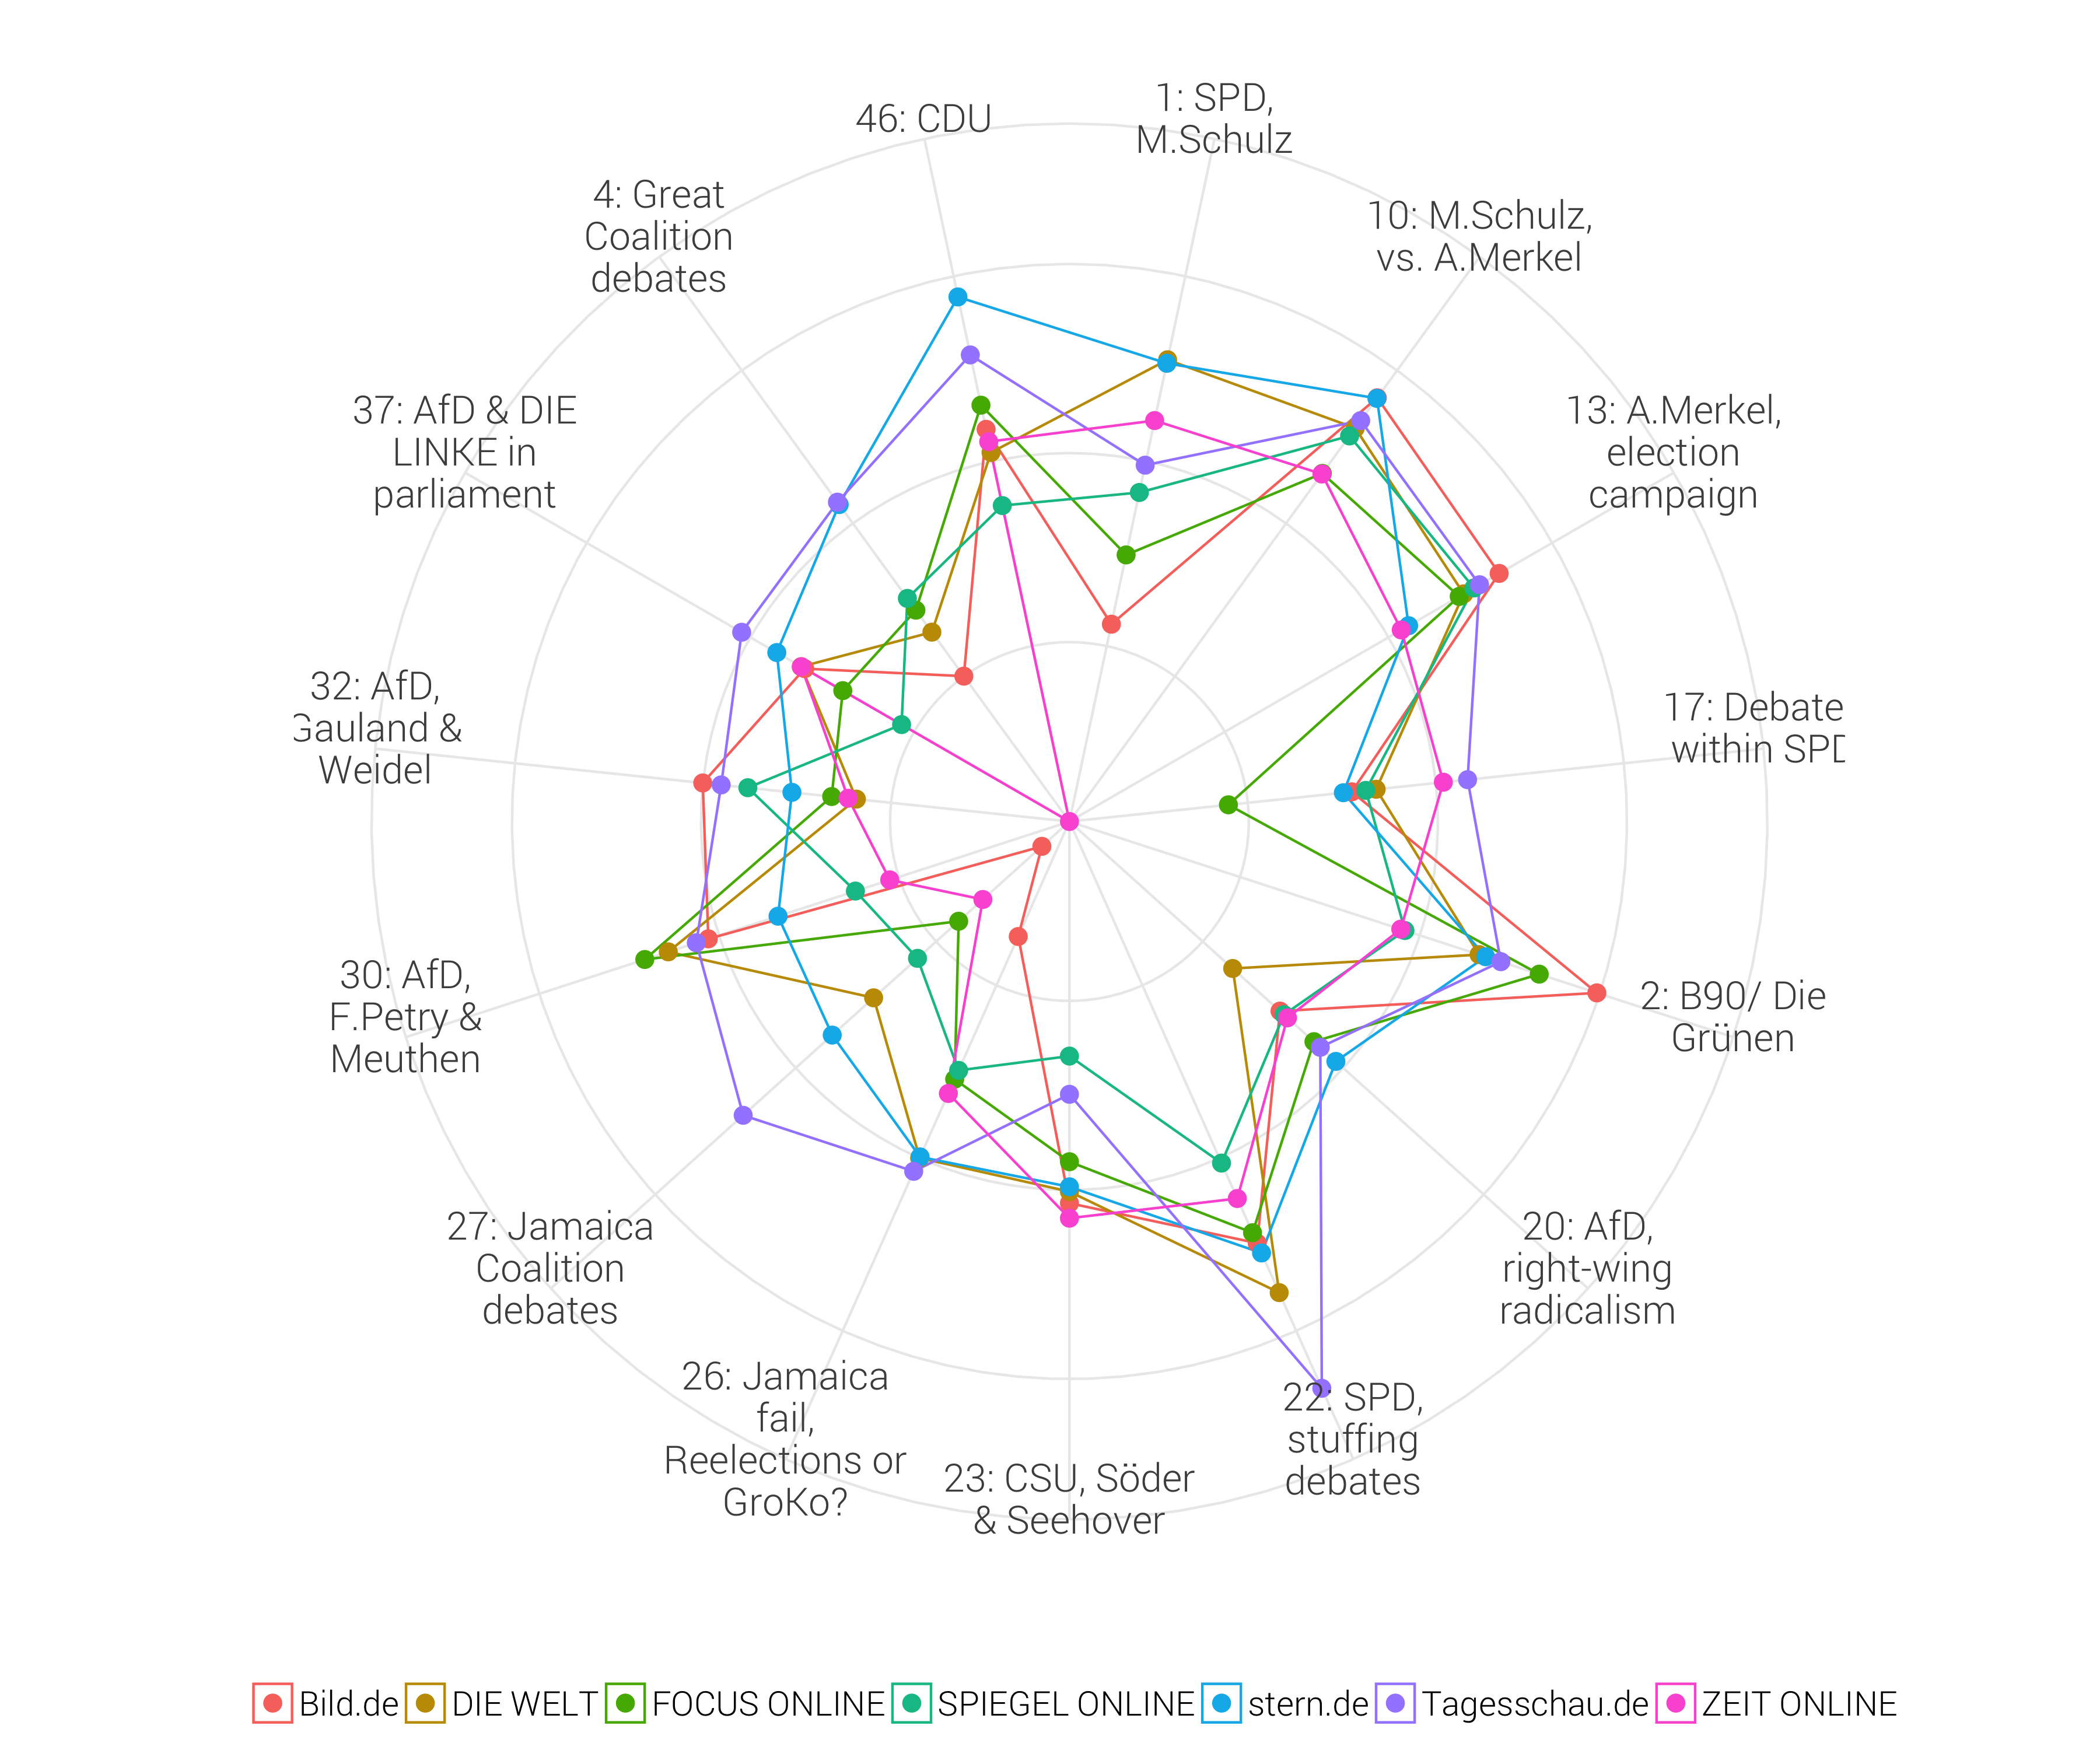
\includegraphics[width=0.8\textwidth,keepaspectratio]{figs/sentscore_radar.png}
			\label{fig_sentscore_radar}
	\end{center}
\end{figure}

After the figures above have been analyzed, the following points can be summarized:

\begin{enumerate}
	\item The sentiment value of the SPD is decreasing over time, especially regarding debates within the party (topic 17). 
	\item The topics relating to the coalition talks on Jamaica (26, 27) and the grand coalition (4) are discussed rather critically, but they also show the greatest differences between the media. 
	\item In contrast, the tonality of the topics in relation to the AfD shows rather small differences. 
	\item Overall, the sentiment value at Tagesschau.de is the least negative and only shows a comparatively strong negative value at topic 23, concerning the CSU.
\end{enumerate} 

\subsection{News sentiment and poll data}\label{ch_correlation}

This section seeks to examine the association between sentiment reflected in online news content and phone poll results in Germany. Specifically, it aims to find the extent to which online sentiment and phone survey results correlate given a number of lags. I use the data from the "Sonntagsumfrage" (Sunday survey) from infratest dimap.\footnote{https://www.infratest-dimap.de/umfragen-analysen/bundesweit/sonntagsfrage/} The institution regularly asks at least 1000 German citizens the question: "Which party would you choose if federal elections were to take place next Sunday?" The survey thus measures the current election tendencies and therefore reflects an intermediate state in the opinion-forming process of the electoral population.

Much of the research on online content and political trends have focused on traditional weblogs and social media websites, such as Twitter, Facebook, MySpace, and YouTube. These studies have shown that social media is used to spread political opinions and that these considerations reflect the political landscape of the offline world. \citet{tumasjan_predicting_2010} investigate Tweets between August 13th and September 19th, 2009, prior to the German national elections to examine whether Twitter messages reflect the current offline political sentiment and whether it can be used to predict the popularity of parties or coalitions in the real world. With regard to the later question, they compare the share of attention the political parties receive on Twitter with the election result to examine whether the activity on Twitter can serve as a predictor of the election outcome. They found that the number of tweets reflects the election result and even comes close to traditional election polls.

\citet{fu_analyzing_2013} use a corpus of online posts from discussion forums and blogs to examine the extent to which online sentiment reflected in social media content can predict phone survey results in Hong Kong. They build a sentiment classifier conducting a support vector machine analysis on a training set of 2,000 manually labeled posts. In order to evaluate the temporal relationship between the time series of the online sentiment score and the results of the telephone survey, a cross correlation analysis was conducted, using the Box and Jenkins autoregressive integrated moving average (ARIMA) method \citep{box_time_2008}. Estimating the cross-correlation functions of the residuals, they find that online sentiment scores can lead phone survey results by about 8–15 days. 

In a more recent conference paper, \citet{padmaja_evaluating_2014} identify the scope of negation in news articles for two political parties in India (BJP and UPA) to analyze how the choice of certain words used in these texts influence the sentiments of public in polls. Comparing three different sentiment analysis methods (two machine learning and one dictionary method), they observe that the choice of certain words used in political text was influencing the sentiments in favor of BJP. They conclude that this sentiment bias might be one of the causes for the election results in 2014.

\citet{dewenter_can_2018} use human-coded data from leading media in Germany together with the German Politbarometer survey to investigate how media coverage affects short- and long-term political preferences between February 1998 and December 2012. They find a positive correlation between the media coverage and the short-term voting intention for a political party. In the long-term, however, voting preferences are stable. 

In the present paper, the relationship between monthly average of both the sentiment value of individual topics ($x_t$) and the survey value of the parties ($y_t$) is estimated using the cross correlation function (CCF). Thus, the CCF between $x_{t+h}$ and $y_t$ for $h\pm 1$,$h \pm 2$,$h \pm 3$ is computed. A negative value for $h$ is a correlation between the topic sentiment value at a time before $t$ and the survey value at time $t$. The correlation value for $h=0$ indicates the contemporary correlation between the two time series.  Based on the coefficients of the cross correlation estimation shown in Figure \ref{fig_ccf}, the significant correlations between topic sentiment and survey value are evaluated for each party.\footnote{The value of the cross correlation coefficients for lag 0 are listed in the appendix \ref{apx_ccf}} It is important to note that no causal relationships are described below, but only the correlation between the two time series. 

The survey results of the AfD correlate negatively with topics relating to the SPD (17, 22) at lag 0. Thus, if the SPD was more negatively reported, the poll value of the AfD increased in the same month (and vice versa). Another significant negative correlation exists between the reporting on the GroKo (4) and the survey value of AfD at lag -1 ($x_{t-1}$). So if the GroKo was more negatively reported in one month, the survey value of the AfD increased in the following month (and vice versa). For the FDP, too, only negative correlation coefficients can be detected, with the strongest negative correlation existing for the topic relating to the CSU (23). If the CSU got off worse in the online news, the poll value of the FDP went up. Another interesting observation is that the FDP's poll results correlate negatively with issues relating to the Jamaica coalition at lag 1 ($x_{t+1}$). So if the poll results for the FDP rose in one month, the following month the FDP was reported more negatively. The Green Party survey results show no negative correlation with any of the topics, except topic 30 at lag 1. It is striking that there seems to be a strong negative correlation between the SPD topics (1, 17, 22) and the poll results of the left party (DIE LINKE). This means that the poll value of the left party has climbed if the topics related to the SPD were discussed more negatively. Same applies to the reporting on the GroKo (30) for lag -1. Conversely, the SPD's survey results correlate strongly positively with these topics, and also with topic 30 with a delay of one month. For the CDU/CSU, too, only significant negative correlations are discernible: the survey results correlate negatively with the topic of the Schulz v Merkel debate (10) and negatively with topic 30 with a delay of one month ($x_{t+1}$). 

\begin{landscape}
\begin{figure}[H]
	\caption{Cross-Correlation Coefficients}
	\begin{center}
			\includegraphics[width=1.3\textwidth,keepaspectratio]{figs/ccf2.png}
			\label{fig_ccf}
	\end{center}
\end{figure} 
\end{landscape}

After the figures above have been analyzed, the following points can be summarized:

\begin{enumerate}
	\item Only the survey results of the SPD correlate positively with the emotional value of the topics. There seems to be a strong correlation between the way topics concerning the SPD are discussed in the online news and the poll results.  
	\item The poll results of the Left Party, on the other hand, seem to correlate negatively with the reporting on the SPD. 
	\item Similar tendencies can also be seen with regard to the AfD, since here too the survey results correlate significantly negatively with the topics about the SPD and the grand coalition. 
\end{enumerate} 

Summarizing the analyses from this and the previous section, it can be observed that the positive correlation between the emotional value of the reporting and the survey value of a party is particularly large if the reporting is conspicuously negative. 

\section{Conclusion}

The ongoing discussion about the influence of digital media on the political opinion-forming process addresses the question whether there are convergence tendencies within the mass media and whether the reporting in the media correlates with the voting preferences. To analyze this question, this paper examines (1) whether the political reporting of different media differs in terms of topic frequency and topic tonality and (2) whether the emotional value of the reporting correlates with poll results. 

Using text data of 14,937 online news articles from seven German news providers about domestic politics, I first estimate a Structural Topic Model to find the latent topics in the news articles in order to answer (1). After assigning a topic to each news article, the sentiment value of articles about contemporary political events is calculated using a dictionary-based method. In order to tackle (2), the results from the sentiment analysis are then compared to poll results.

Regarding (1), the analysis revealed that there are differences between the media considered, both in terms of topic prevalence and the way in which these topics are discussed. Although the topics are discussed negatively on average, differences can still be observed, especially regarding topics that deal with the coalition negotiations. The smallest differences were observed for topics concerning the AfD. However, no evidence has been found that the media systematically report more negatively on the AfD than on other parties. With regard to (2), the analysis has shown that the tonality of topics discussed by the SPD shows a strong positive correlation to current survey results. Overall, there seems to be a link between reporting on political issues and electoral preferences. The results of this study show evidence that the content of media could have an influence on the opinion-forming process of the voters and therefore underline the responsibility of media in the political context.

\pagebreak

\printbibliography

\appendix
\section{Appendices}

\subsection{Generative Process of STM}\label{ch_generativeProcess}

 The following describes the generative process for filling the $n^{th}$ word-position in document $d$ in the case of the STM \citep{roberts_structural_2013}: As in the case of conventional models, first a specific topic $z_{dn}$ is assigned, according to the topic distribution for that document $\theta$ through the process:

\begin{equation}
	z_{dn}|\theta_d \sim \textrm{Multinomial}(\theta_d).
\end{equation}

To incorporate the covariate values for that document, a topic-prevalence vector $\theta_d$ is drawn from a logistic-normal distribution:

\begin{equation}
	\theta_d|y_{d\gamma},\Sigma \sim \textrm{LogisticNormal}(\mu = y_{d\gamma}\Sigma),
\end{equation}

where $y_d\gamma$ lists the values of the metadata covariates for document $d$ and $\gamma$ relates these covariate values to the topic-prevalence. 

Conditional in the topic chosen ($z_{dn}$), a specific word $w_{dn}$, is selected from the overall corpus vocabulary $V$, using the following process:

\begin{equation}
	w_{dn}|z_{dn},\phi_{dkv} \sim \textrm{Multinomial}(\phi_{dk1},...,\phi_{dkV}),
\end{equation}

where the word probability $\phi_{dkv}$ is parameterized in terms of log-transformed rate deviations from the rates of a corpus-wide background distribution $m_v$ \citep{roberts_structural_2013}. The log-transformed rate deviations can then be specified by a collection of parameters $\lbrace \boldsymbol{\kappa} \rbrace$, where $\kappa^{(t)}$ is a $K$-by-$V$ matrix containing the log-transformed rate deviations for each topic $k$ and term $v$, over the baseline log-transformed rate for term $v$. This matrix is the same for all $A$ levels of covariates. To put it differently, $\kappa^{(t)}$ indicates the importance of the term $v$ given topic $k$ regardless of the covariates. Similarly, $\kappa^{(c)}$ is a $A$-by-$V$ matrix, indicating the importance of the term $v$ given the covariate level $c$ regardless of the topic. Finally, $\kappa^{(i)}$ is a $A$-by-$K$-by-$V$ matrix, collecting the covariate-topic effects:

\begin{equation}
	\phi_{dkv}|z_{dn}=\frac{\textrm{exp}(m_v+\kappa^{(t)}_{kv},\kappa^{(c)}_{y_dv}+\kappa^{(i)}_{y_dkv})}{\sum_v \textrm{exp}(m_v+\kappa^{(t)}_{kv},\kappa^{(c)}_{y_dv}+\kappa^{(i)}_{y_dkv})}.
\end{equation}

The STM maximizes the posterior likelihood that the observed data were generated by the above data-generating process using an iterative approximation-based variational expectation-maximization algorithm\footnote{A technical description of this maximization process can be found in \citet{roberts_model_2016}} available in R's stm package \citep{roberts_stm:_2016}. 

This process generates two posterior distribution parameters: 

\begin{enumerate}
	\item $\phi$ is a $K$-by-$V$ matrix (where $K=$ number of topics and $V=$ vocabulary or unique terms), where the entry $\phi_{kvc}$ can be interpreted as the probability of observing the $v$-th word in topic $k$ for the covariate level $c$ (the news website). 
	\item $\theta$ is a $D$-by-$V$ matrix (where $D=$ number of documents and $V=$ vocabulary or unique terms) of the document-topic distributions, where the entry $\theta_{dk}$ can be interpreted as the proportion of words in document $d$ which arise from topic $k$, or rather as the probability that document $d$ deals about topic $k$. 
\end{enumerate}


\subsection{Wordclouds}\label{apx_wordclouds}
\begin{figure}[H]
	\begin{center}
		\begin{subfigure}[normla]{0.43\textwidth}
			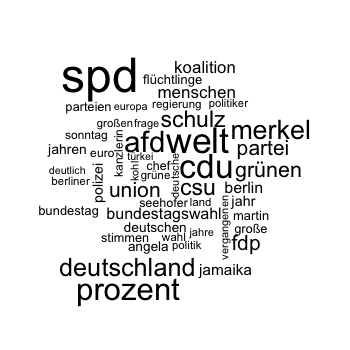
\includegraphics[width=\textwidth]{figs/wordcloud_DIEWELT.png}
			\caption{DIE WELT}
		\end{subfigure}
		\begin{subfigure}[normla]{0.43\textwidth}
			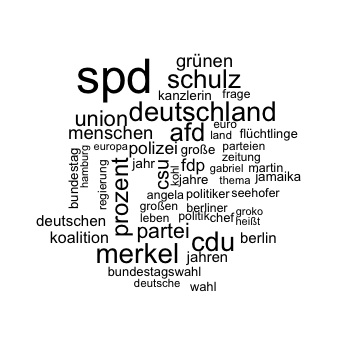
\includegraphics[width=\textwidth]{figs/wordcloud_FOCUSONLINE.png}
			\caption{FOCUS ONLINE}
		\end{subfigure}
		\begin{subfigure}[normla]{0.43\textwidth}
			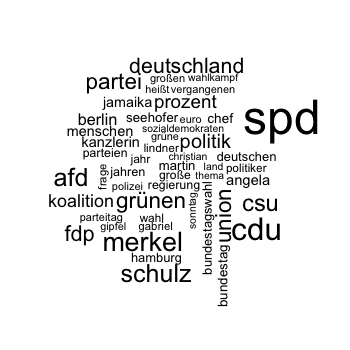
\includegraphics[width=\textwidth]{figs/wordcloud_SPIEGELONLINE.png}
			\caption{SPIEGEL ONLINE}
		\end{subfigure}
		\begin{subfigure}[normla]{0.43\textwidth}
			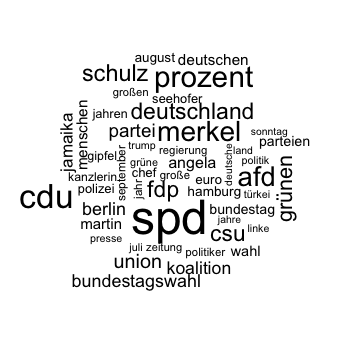
\includegraphics[width=\textwidth]{figs/wordcloud_stern.png}
			\caption{Stern.de}
		\end{subfigure}
		\begin{subfigure}[normla]{0.43\textwidth}
			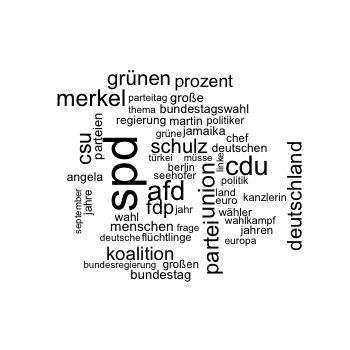
\includegraphics[width=\textwidth]{figs/wordcloud_ZEITONLINE.png}
			\caption{ZEIT ONLINE}
		\end{subfigure}
	\end{center}
\end{figure}

\subsection{Most frequent words}\label{apx_tf}
% 1, 2
\begin{figure}[H]
	\begin{center}
		\begin{subfigure}[normla]{0.49\textwidth}
			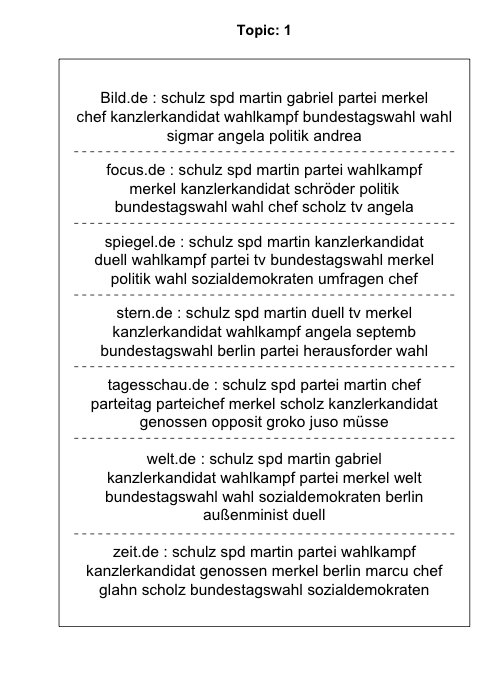
\includegraphics[width=\textwidth]{figs/plotquote1.png}
		\end{subfigure}
		\begin{subfigure}[normla]{0.49\textwidth}
			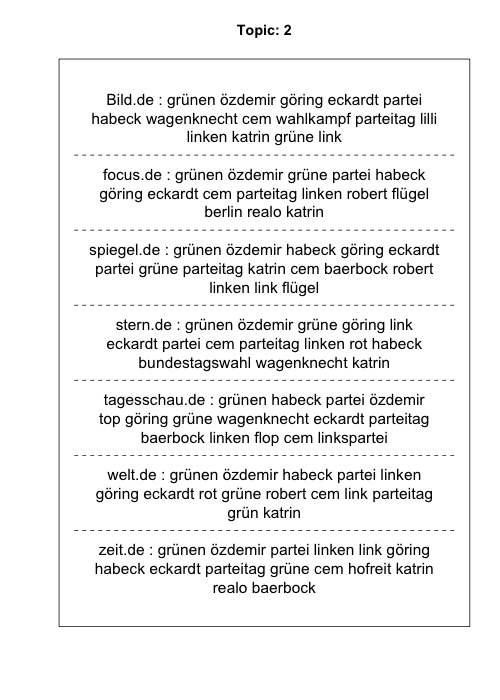
\includegraphics[width=\textwidth]{figs/plotquote2.png}
		\end{subfigure}
	\end{center}
\end{figure}
	
% 4, 10
\begin{figure}[H]
	\begin{center}
		\begin{subfigure}[normla]{0.49\textwidth}
			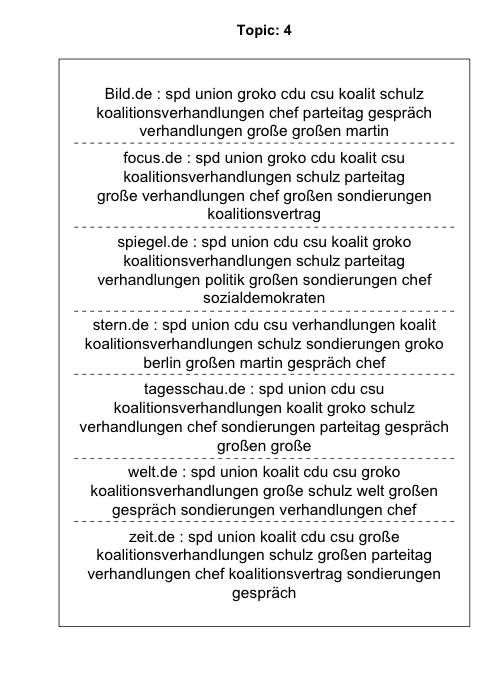
\includegraphics[width=\textwidth]{figs/plotquote4.png}
		\end{subfigure}
		\begin{subfigure}[normla]{0.49\textwidth}
			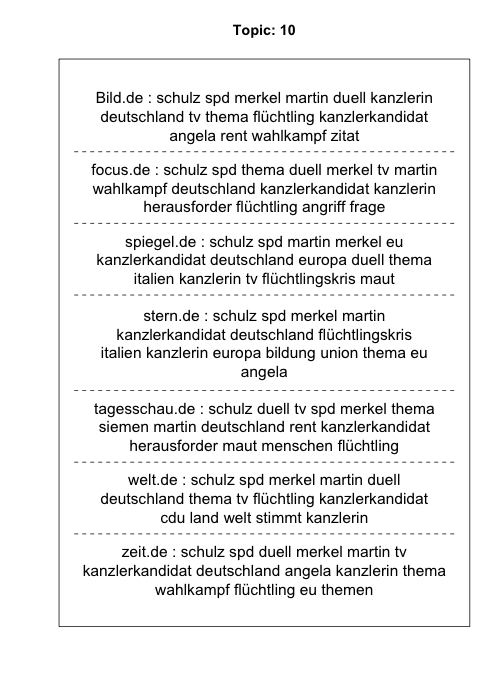
\includegraphics[width=\textwidth]{figs/plotquote10.png}
		\end{subfigure}
	\end{center}
\end{figure}

% 13, 17
\begin{figure}[H]
	\begin{center}
		\begin{subfigure}[normla]{0.49\textwidth}
			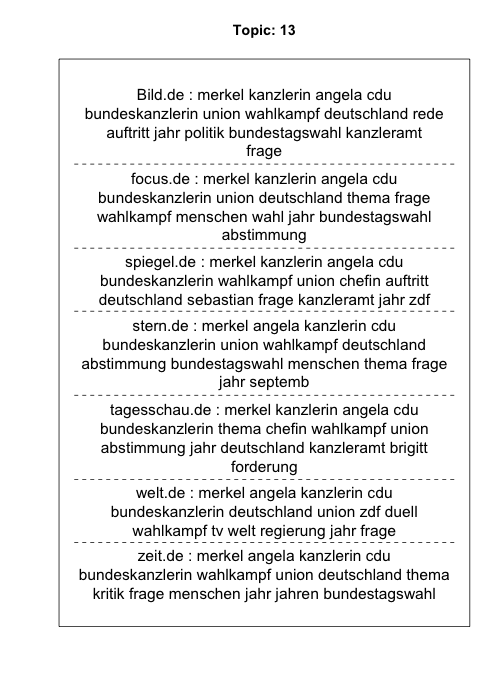
\includegraphics[width=\textwidth]{figs/plotquote13.png}
		\end{subfigure}
		\begin{subfigure}[normla]{0.49\textwidth}
			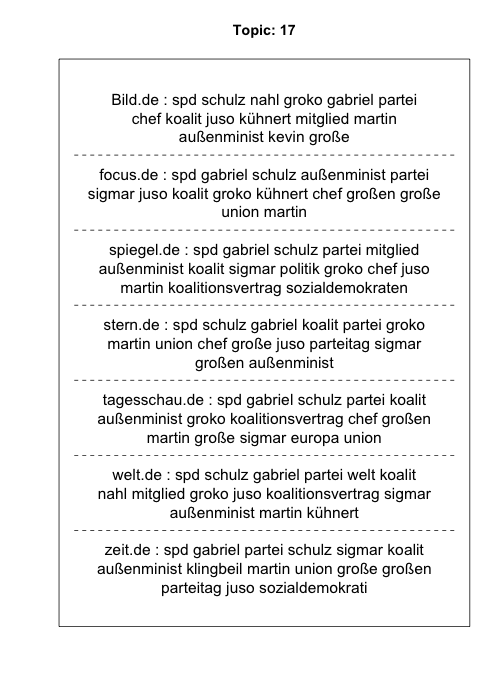
\includegraphics[width=\textwidth]{figs/plotquote17.png}
		\end{subfigure}
	\end{center}
\end{figure}

% 20, 23
\begin{figure}[H]
	\begin{center}
		\begin{subfigure}[normla]{0.49\textwidth}
			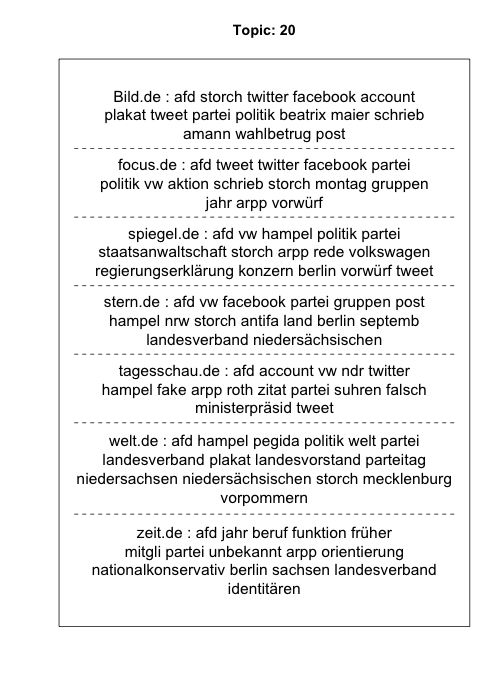
\includegraphics[width=\textwidth]{figs/plotquote20.png}
		\end{subfigure}
		\begin{subfigure}[normla]{0.49\textwidth}
			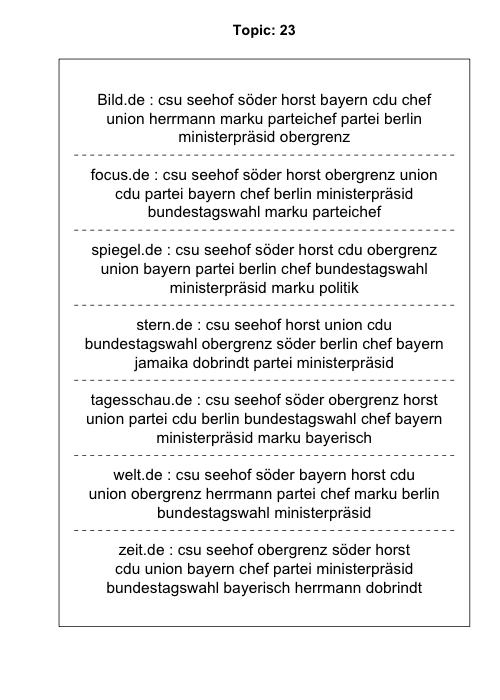
\includegraphics[width=\textwidth]{figs/plotquote23.png}
		\end{subfigure}
	\end{center}
\end{figure}

% 26, 27
\begin{figure}[H]
	\begin{center}
		\begin{subfigure}[normla]{0.49\textwidth}
			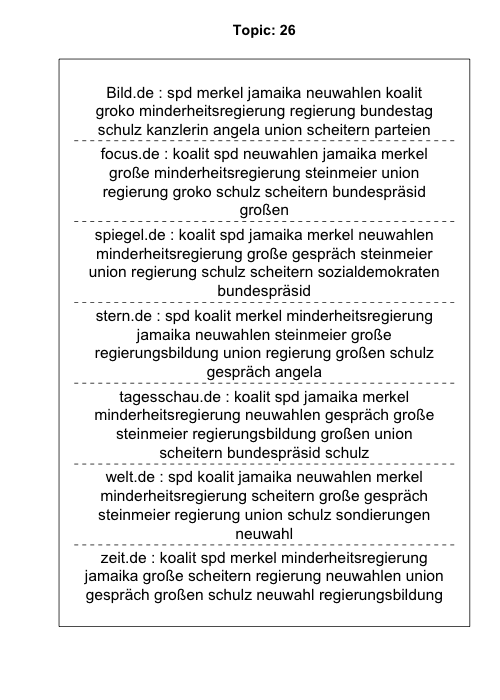
\includegraphics[width=\textwidth]{figs/plotquote26.png}
		\end{subfigure}
		\begin{subfigure}[normla]{0.49\textwidth}
			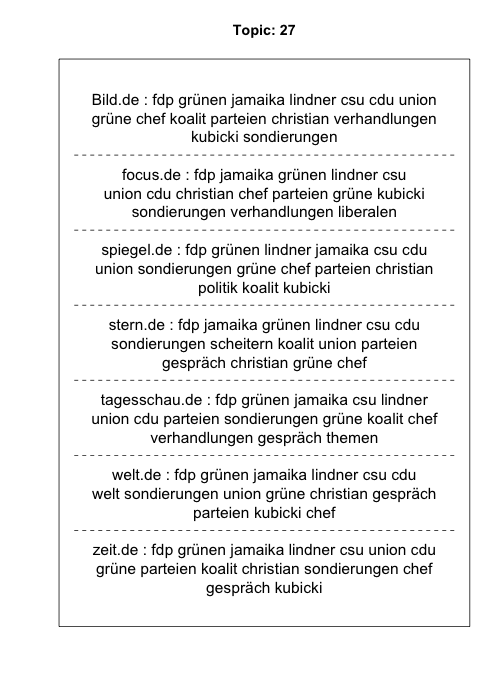
\includegraphics[width=\textwidth]{figs/plotquote27.png}
		\end{subfigure}
	\end{center}
\end{figure}

% 30, 32
\begin{figure}[H]
	\begin{center}
		\begin{subfigure}[normla]{0.49\textwidth}
			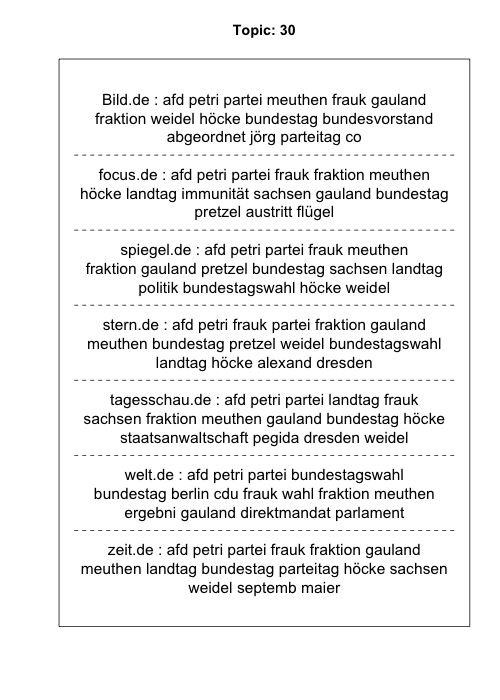
\includegraphics[width=\textwidth]{figs/plotquote30.png}
		\end{subfigure}
		\begin{subfigure}[normla]{0.49\textwidth}
			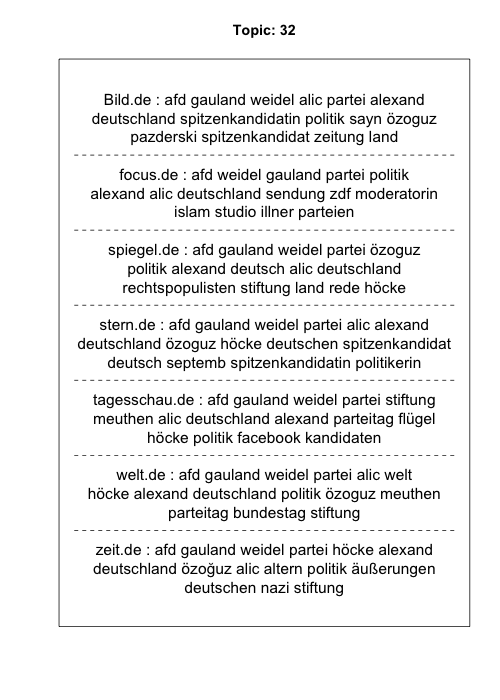
\includegraphics[width=\textwidth]{figs/plotquote32.png}
		\end{subfigure}
	\end{center}
\end{figure}

% 37, 46
\begin{figure}[H]
	\begin{center}
		\begin{subfigure}[normla]{0.49\textwidth}
			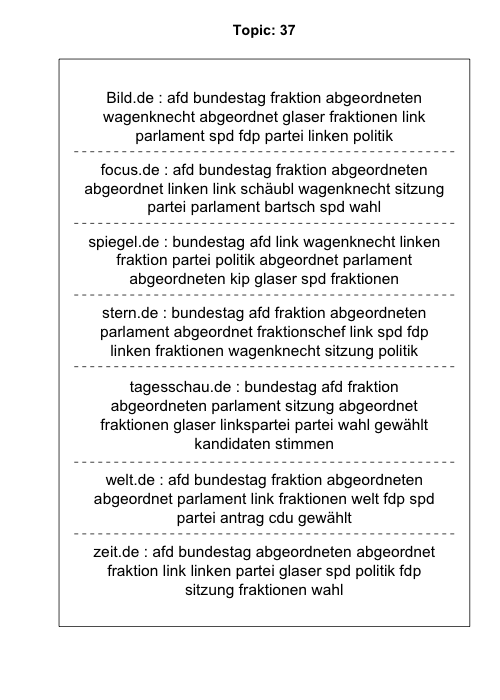
\includegraphics[width=\textwidth]{figs/plotquote37.png}
		\end{subfigure}
		\begin{subfigure}[normla]{0.49\textwidth}
			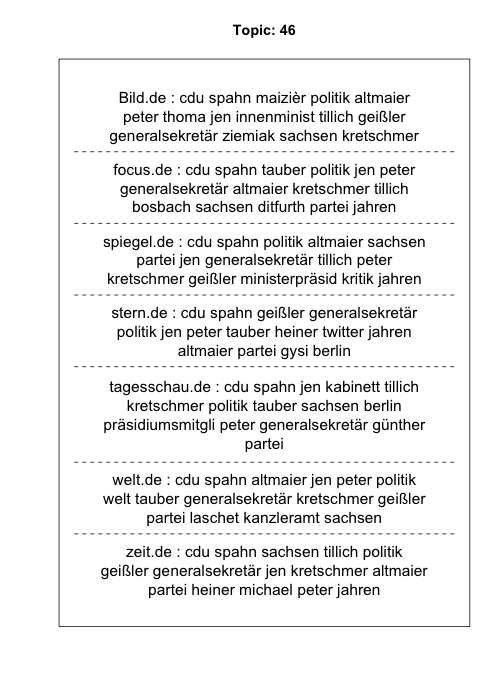
\includegraphics[width=\textwidth]{figs/plotquote46.png}
		\end{subfigure}
	\end{center}
\end{figure}

\subsection{Regression Results}\label{apx_coeff}
\begin{minipage}[t]{0.49\textwidth}
	% latex table generated in R 3.4.2 by xtable 1.8-2 package
% Tue May  8 10:07:43 2018
\begin{adjustbox}{width=\textwidth,totalheight=\textheight,keepaspectratio}
\begin{tabular}{llrrrr}
  \hline
topic\_name & parameter & Estimate & Std. Error & t value & p \\ 
  \hline
1: SPD, M.Schulz & (Intercept) & 0.036 & 0.003 & 11.460 & 0.000 \\ 
  1: SPD, M.Schulz & FOCUS ONLINE & -0.007 & 0.004 & -1.777 & 0.076 \\ 
  1: SPD, M.Schulz & SPIEGEL ONLINE & -0.008 & 0.004 & -1.965 & 0.049 \\ 
  1: SPD, M.Schulz & stern.de & -0.009 & 0.004 & -2.340 & 0.019 \\ 
  1: SPD, M.Schulz & Tagesschau.de & -0.015 & 0.005 & -3.311 & 0.001 \\ 
  1: SPD, M.Schulz & DIE WELT & -0.015 & 0.004 & -3.834 & 0.000 \\ 
  1: SPD, M.Schulz & ZEIT ONLINE & -0.012 & 0.004 & -2.686 & 0.007 \\ 
  2: B90/ Die Grünen & (Intercept) & 0.018 & 0.003 & 7.057 & 0.000 \\ 
  2: B90/ Die Grünen & FOCUS ONLINE & -0.005 & 0.003 & -1.515 & 0.130 \\ 
  2: B90/ Die Grünen & SPIEGEL ONLINE & 0.001 & 0.003 & 0.260 & 0.795 \\ 
  2: B90/ Die Grünen & stern.de & 0.005 & 0.003 & 1.689 & 0.091 \\ 
  2: B90/ Die Grünen & Tagesschau.de & -0.003 & 0.004 & -0.805 & 0.421 \\ 
  2: B90/ Die Grünen & DIE WELT & -0.004 & 0.003 & -1.160 & 0.246 \\ 
  2: B90/ Die Grünen & ZEIT ONLINE & 0.004 & 0.004 & 1.035 & 0.301 \\ 
  4: Great Coalition debates & (Intercept) & 0.064 & 0.005 & 13.210 & 0.000 \\ 
  4: Great Coalition debates & FOCUS ONLINE & -0.010 & 0.006 & -1.698 & 0.089 \\ 
  4: Great Coalition debates & SPIEGEL ONLINE & 0.003 & 0.006 & 0.487 & 0.626 \\ 
  4: Great Coalition debates & stern.de & -0.032 & 0.006 & -5.472 & 0.000 \\ 
  4: Great Coalition debates & Tagesschau.de & -0.005 & 0.006 & -0.841 & 0.401 \\ 
  4: Great Coalition debates & DIE WELT & -0.012 & 0.006 & -2.183 & 0.029 \\ 
  4: Great Coalition debates & ZEIT ONLINE & 0.002 & 0.006 & 0.400 & 0.689 \\ 
  10: M.Schulz, vs. A.Merkel & (Intercept) & 0.009 & 0.002 & 4.131 & 0.000 \\ 
  10: M.Schulz, vs. A.Merkel & FOCUS ONLINE & 0.001 & 0.003 & 0.192 & 0.848 \\ 
  10: M.Schulz, vs. A.Merkel & SPIEGEL ONLINE & 0.002 & 0.003 & 0.565 & 0.572 \\ 
  10: M.Schulz, vs. A.Merkel & stern.de & 0.007 & 0.003 & 2.860 & 0.004 \\ 
  10: M.Schulz, vs. A.Merkel & Tagesschau.de & 0.003 & 0.003 & 0.991 & 0.322 \\ 
  10: M.Schulz, vs. A.Merkel & DIE WELT & -0.003 & 0.003 & -1.117 & 0.264 \\ 
  10: M.Schulz, vs. A.Merkel & ZEIT ONLINE & 0.012 & 0.003 & 3.798 & 0.000 \\ 
  13: A.Merkel, election campaign & (Intercept) & 0.024 & 0.003 & 9.704 & 0.000 \\ 
  13: A.Merkel, election campaign & FOCUS ONLINE & 0.002 & 0.003 & 0.550 & 0.582 \\ 
  13: A.Merkel, election campaign & SPIEGEL ONLINE & 0.003 & 0.003 & 0.992 & 0.321 \\ 
  13: A.Merkel, election campaign & stern.de & 0.009 & 0.003 & 2.709 & 0.007 \\ 
  13: A.Merkel, election campaign & Tagesschau.de & -0.006 & 0.003 & -1.824 & 0.068 \\ 
  13: A.Merkel, election campaign & DIE WELT & 0.001 & 0.003 & 0.297 & 0.767 \\ 
  13: A.Merkel, election campaign & ZEIT ONLINE & 0.004 & 0.004 & 1.137 & 0.256 \\ 
  17: Debates within SPD & (Intercept) & 0.035 & 0.003 & 10.632 & 0.000 \\ 
  17: Debates within SPD & FOCUS ONLINE & -0.005 & 0.004 & -1.315 & 0.189 \\ 
  17: Debates within SPD & SPIEGEL ONLINE & -0.009 & 0.004 & -2.186 & 0.029 \\ 
  17: Debates within SPD & stern.de & -0.001 & 0.004 & -0.361 & 0.718 \\ 
  17: Debates within SPD & Tagesschau.de & -0.013 & 0.005 & -2.809 & 0.005 \\ 
  17: Debates within SPD & DIE WELT & -0.010 & 0.004 & -2.612 & 0.009 \\ 
  17: Debates within SPD & ZEIT ONLINE & -0.007 & 0.005 & -1.579 & 0.114 \\ 
  20: AfD, right-wing radicalism & (Intercept) & 0.017 & 0.003 & 5.704 & 0.000 \\ 
  20: AfD, right-wing radicalism & FOCUS ONLINE & -0.002 & 0.004 & -0.607 & 0.544 \\ 
  20: AfD, right-wing radicalism & SPIEGEL ONLINE & -0.003 & 0.004 & -0.724 & 0.469 \\ 
  20: AfD, right-wing radicalism & stern.de & -0.003 & 0.004 & -0.784 & 0.433 \\ 
  20: AfD, right-wing radicalism & Tagesschau.de & -0.000 & 0.004 & -0.033 & 0.973 \\ 
  20: AfD, right-wing radicalism & DIE WELT & 0.002 & 0.004 & 0.512 & 0.609 \\ 
  20: AfD, right-wing radicalism & ZEIT ONLINE & -0.002 & 0.004 & -0.538 & 0.590 \\ 
  22: SPD, stuffing debates & (Intercept) & 0.019 & 0.003 & 7.408 & 0.000 \\ 
  22: SPD, stuffing debates & FOCUS ONLINE & -0.004 & 0.003 & -1.170 & 0.242 \\ 
  22: SPD, stuffing debates & SPIEGEL ONLINE & 0.010 & 0.003 & 2.960 & 0.003 \\ 
  22: SPD, stuffing debates & stern.de & -0.006 & 0.003 & -1.943 & 0.052 \\ 
  22: SPD, stuffing debates & Tagesschau.de & -0.003 & 0.003 & -0.903 & 0.367 \\ 
  22: SPD, stuffing debates & DIE WELT & -0.004 & 0.003 & -1.308 & 0.191 \\ 
  22: SPD, stuffing debates & ZEIT ONLINE & 0.005 & 0.003 & 1.449 & 0.147 \\ 
   \hline
\end{tabular}
\end{adjustbox}

\end{minipage}
\begin{minipage}[t]{0.49\textwidth}
	% latex table generated in R 3.4.2 by xtable 1.8-2 package
% Tue May  8 10:07:44 2018
\begin{adjustbox}{width=\textwidth,totalheight=\textheight,keepaspectratio}
\begin{tabular}{llrrrr}
  \hline
topic\_name & parameter & Estimate & Std. Error & t value & p \\ 
  \hline
23: CSU, Söder \& Seehover & (Intercept) & 0.035 & 0.004 & 9.191 & 0.000 \\ 
  23: CSU, Söder \& Seehover & FOCUS ONLINE & -0.004 & 0.005 & -0.887 & 0.375 \\ 
  23: CSU, Söder \& Seehover & SPIEGEL ONLINE & 0.006 & 0.005 & 1.094 & 0.274 \\ 
  23: CSU, Söder \& Seehover & stern.de & -0.002 & 0.005 & -0.365 & 0.715 \\ 
  23: CSU, Söder \& Seehover & Tagesschau.de & -0.006 & 0.005 & -1.214 & 0.225 \\ 
  23: CSU, Söder \& Seehover & DIE WELT & -0.006 & 0.004 & -1.238 & 0.216 \\ 
  23: CSU, Söder \& Seehover & ZEIT ONLINE & 0.002 & 0.005 & 0.357 & 0.721 \\ 
  26: Jamaica fail, Reelections or GroKo? & (Intercept) & 0.035 & 0.003 & 11.775 & 0.000 \\ 
  26: Jamaica fail, Reelections or GroKo? & FOCUS ONLINE & -0.004 & 0.004 & -1.137 & 0.256 \\ 
  26: Jamaica fail, Reelections or GroKo? & SPIEGEL ONLINE & -0.004 & 0.004 & -1.076 & 0.282 \\ 
  26: Jamaica fail, Reelections or GroKo? & stern.de & -0.012 & 0.004 & -3.463 & 0.001 \\ 
  26: Jamaica fail, Reelections or GroKo? & Tagesschau.de & -0.010 & 0.004 & -2.584 & 0.010 \\ 
  26: Jamaica fail, Reelections or GroKo? & DIE WELT & -0.012 & 0.004 & -3.333 & 0.001 \\ 
  26: Jamaica fail, Reelections or GroKo? & ZEIT ONLINE & -0.005 & 0.004 & -1.356 & 0.175 \\ 
  27: Jamaica Coalition debates & (Intercept) & 0.066 & 0.005 & 13.865 & 0.000 \\ 
  27: Jamaica Coalition debates & FOCUS ONLINE & -0.029 & 0.006 & -5.152 & 0.000 \\ 
  27: Jamaica Coalition debates & SPIEGEL ONLINE & -0.009 & 0.006 & -1.438 & 0.150 \\ 
  27: Jamaica Coalition debates & stern.de & -0.028 & 0.006 & -5.088 & 0.000 \\ 
  27: Jamaica Coalition debates & Tagesschau.de & -0.018 & 0.006 & -2.939 & 0.003 \\ 
  27: Jamaica Coalition debates & DIE WELT & -0.008 & 0.005 & -1.416 & 0.157 \\ 
  27: Jamaica Coalition debates & ZEIT ONLINE & -0.003 & 0.007 & -0.460 & 0.645 \\ 
  30: AfD, F.Petry \& Meuthen & (Intercept) & 0.026 & 0.003 & 7.579 & 0.000 \\ 
  30: AfD, F.Petry \& Meuthen & FOCUS ONLINE & -0.005 & 0.004 & -1.168 & 0.243 \\ 
  30: AfD, F.Petry \& Meuthen & SPIEGEL ONLINE & 0.002 & 0.004 & 0.430 & 0.667 \\ 
  30: AfD, F.Petry \& Meuthen & stern.de & -0.004 & 0.004 & -0.896 & 0.370 \\ 
  30: AfD, F.Petry \& Meuthen & Tagesschau.de & -0.014 & 0.004 & -3.035 & 0.002 \\ 
  30: AfD, F.Petry \& Meuthen & DIE WELT & -0.011 & 0.004 & -2.812 & 0.005 \\ 
  30: AfD, F.Petry \& Meuthen & ZEIT ONLINE & 0.004 & 0.005 & 0.914 & 0.361 \\ 
  32: AfD, Gauland \& Weidel & (Intercept) & 0.023 & 0.004 & 6.308 & 0.000 \\ 
  32: AfD, Gauland \& Weidel & FOCUS ONLINE & 0.001 & 0.004 & 0.191 & 0.848 \\ 
  32: AfD, Gauland \& Weidel & SPIEGEL ONLINE & -0.001 & 0.005 & -0.123 & 0.902 \\ 
  32: AfD, Gauland \& Weidel & stern.de & 0.007 & 0.004 & 1.593 & 0.111 \\ 
  32: AfD, Gauland \& Weidel & Tagesschau.de & -0.006 & 0.005 & -1.221 & 0.222 \\ 
  32: AfD, Gauland \& Weidel & DIE WELT & 0.006 & 0.004 & 1.378 & 0.168 \\ 
  32: AfD, Gauland \& Weidel & ZEIT ONLINE & 0.006 & 0.005 & 1.198 & 0.231 \\ 
  37: AfD \& DIE LINKE in parliament & (Intercept) & 0.024 & 0.004 & 6.652 & 0.000 \\ 
  37: AfD \& DIE LINKE in parliament & FOCUS ONLINE & 0.005 & 0.004 & 1.221 & 0.222 \\ 
  37: AfD \& DIE LINKE in parliament & SPIEGEL ONLINE & 0.013 & 0.005 & 2.984 & 0.003 \\ 
  37: AfD \& DIE LINKE in parliament & stern.de & 0.001 & 0.004 & 0.252 & 0.801 \\ 
  37: AfD \& DIE LINKE in parliament & Tagesschau.de & 0.005 & 0.005 & 1.130 & 0.258 \\ 
  37: AfD \& DIE LINKE in parliament & DIE WELT & 0.002 & 0.004 & 0.483 & 0.629 \\ 
  37: AfD \& DIE LINKE in parliament & ZEIT ONLINE & 0.011 & 0.005 & 2.143 & 0.032 \\ 
  46: CDU & (Intercept) & 0.018 & 0.002 & 7.336 & 0.000 \\ 
  46: CDU & FOCUS ONLINE & -0.001 & 0.003 & -0.245 & 0.806 \\ 
  46: CDU & SPIEGEL ONLINE & 0.002 & 0.003 & 0.753 & 0.451 \\ 
  46: CDU & stern.de & -0.006 & 0.003 & -1.942 & 0.052 \\ 
  46: CDU & Tagesschau.de & -0.011 & 0.003 & -3.364 & 0.001 \\ 
  46: CDU & DIE WELT & -0.001 & 0.003 & -0.403 & 0.687 \\ 
  46: CDU & ZEIT ONLINE & -0.000 & 0.003 & -0.023 & 0.982 \\ 
   \hline
\end{tabular}
\end{adjustbox}

\end{minipage}

\subsection{Sentiment Values (monthly aggregated)}\label{apx_sentscore_monthly}

\begin{minipage}[t]{0.49\textwidth}
	% latex table generated in R 3.4.2 by xtable 1.8-2 package
% Tue May  8 10:36:37 2018
\begin{adjustbox}{width=\textwidth}
\begin{tabular}{llrr}
  \hline
date & topic & Number of Obs. & sentiment value * 1000 \\ 
  \hline
2017-06-01 & 1: SPD, M.Schulz &  51 & -0.04 \\ 
  2017-07-01 & 1: SPD, M.Schulz &  20 & -0.01 \\ 
  2017-08-01 & 1: SPD, M.Schulz &  49 & -0.02 \\ 
  2017-09-01 & 1: SPD, M.Schulz & 103 & -0.05 \\ 
  2017-10-01 & 1: SPD, M.Schulz &  42 & -0.01 \\ 
  2017-11-01 & 1: SPD, M.Schulz &  34 & -0.04 \\ 
  2017-12-01 & 1: SPD, M.Schulz &  24 & -0.04 \\ 
  2018-01-01 & 1: SPD, M.Schulz &  29 & -0.02 \\ 
  2018-02-01 & 1: SPD, M.Schulz &  47 & -0.18 \\ 
  2017-06-01 & 2: B90/ Die Grünen &  50 & -0.08 \\ 
  2017-07-01 & 2: B90/ Die Grünen &   8 & -0.00 \\ 
  2017-08-01 & 2: B90/ Die Grünen &   8 & -0.01 \\ 
  2017-09-01 & 2: B90/ Die Grünen &  51 & -0.01 \\ 
  2017-10-01 & 2: B90/ Die Grünen &  12 & -0.02 \\ 
  2017-11-01 & 2: B90/ Die Grünen &  22 & -0.02 \\ 
  2017-12-01 & 2: B90/ Die Grünen &  31 & -0.03 \\ 
  2018-01-01 & 2: B90/ Die Grünen &  59 & -0.06 \\ 
  2018-02-01 & 2: B90/ Die Grünen &   1 & -0.00 \\ 
  2017-06-01 & 4: Great Coalition debates &   1 & -0.00 \\ 
  2017-09-01 & 4: Great Coalition debates &   2 & -0.00 \\ 
  2017-10-01 & 4: Great Coalition debates &   1 & -0.00 \\ 
  2017-11-01 & 4: Great Coalition debates &  84 & -0.07 \\ 
  2017-12-01 & 4: Great Coalition debates & 219 & -0.15 \\ 
  2018-01-01 & 4: Great Coalition debates & 382 & -0.29 \\ 
  2018-02-01 & 4: Great Coalition debates & 119 & -0.03 \\ 
  2017-06-01 & 10: M.Schulz, vs. A.Merkel &  11 & -0.02 \\ 
  2017-07-01 & 10: M.Schulz, vs. A.Merkel &  50 & -0.06 \\ 
  2017-08-01 & 10: M.Schulz, vs. A.Merkel &  19 & -0.01 \\ 
  2017-09-01 & 10: M.Schulz, vs. A.Merkel &  56 & -0.02 \\ 
  2017-10-01 & 10: M.Schulz, vs. A.Merkel &   1 & -0.00 \\ 
  2017-11-01 & 10: M.Schulz, vs. A.Merkel &   4 & -0.00 \\ 
  2017-12-01 & 10: M.Schulz, vs. A.Merkel &   7 & -0.00 \\ 
  2018-01-01 & 10: M.Schulz, vs. A.Merkel &   5 & -0.01 \\ 
  2018-02-01 & 10: M.Schulz, vs. A.Merkel &   5 & -0.03 \\ 
  2017-06-01 & 13: A.Merkel, election campaign &  56 & -0.04 \\ 
  2017-07-01 & 13: A.Merkel, election campaign &  13 & -0.02 \\ 
  2017-08-01 & 13: A.Merkel, election campaign &  40 & -0.04 \\ 
  2017-09-01 & 13: A.Merkel, election campaign &  98 & -0.05 \\ 
  2017-10-01 & 13: A.Merkel, election campaign &   6 & -0.01 \\ 
  2017-11-01 & 13: A.Merkel, election campaign &  18 & -0.01 \\ 
  2017-12-01 & 13: A.Merkel, election campaign &  17 & -0.01 \\ 
  2018-01-01 & 13: A.Merkel, election campaign &   7 & -0.01 \\ 
  2018-02-01 & 13: A.Merkel, election campaign &  17 & -0.05 \\ 
  2017-06-01 & 17: Debates within SPD &  14 & -0.00 \\ 
  2017-07-01 & 17: Debates within SPD &   1 & -0.00 \\ 
  2017-08-01 & 17: Debates within SPD &   9 & -0.02 \\ 
  2017-09-01 & 17: Debates within SPD &  13 & -0.02 \\ 
  2017-10-01 & 17: Debates within SPD &  13 & -0.01 \\ 
  2017-11-01 & 17: Debates within SPD &  20 & -0.04 \\ 
  2017-12-01 & 17: Debates within SPD &  70 & -0.07 \\ 
  2018-01-01 & 17: Debates within SPD & 122 & -0.16 \\ 
  2018-02-01 & 17: Debates within SPD & 161 & -0.30 \\ 
  2017-06-01 & 20: AfD, right-wing radicalism &  19 & -0.05 \\ 
  2017-07-01 & 20: AfD, right-wing radicalism &  19 & -0.04 \\ 
  2017-08-01 & 20: AfD, right-wing radicalism &  58 & -0.19 \\ 
  2017-09-01 & 20: AfD, right-wing radicalism &  32 & -0.03 \\ 
  2017-10-01 & 20: AfD, right-wing radicalism &  31 & -0.06 \\ 
  2017-11-01 & 20: AfD, right-wing radicalism &  15 & -0.02 \\ 
  2017-12-01 & 20: AfD, right-wing radicalism &  21 & -0.02 \\ 
  2018-01-01 & 20: AfD, right-wing radicalism &  30 & -0.05 \\ 
  2018-02-01 & 20: AfD, right-wing radicalism &  15 & -0.08 \\ 
  2017-06-01 & 22: SPD, stuffing debates &   4 & -0.00 \\ 
  2017-07-01 & 22: SPD, stuffing debates &  11 & 0.01 \\ 
  2017-08-01 & 22: SPD, stuffing debates &   4 & -0.00 \\ 
  2017-09-01 & 22: SPD, stuffing debates &  43 & -0.04 \\ 
  2017-10-01 & 22: SPD, stuffing debates &  34 & -0.03 \\ 
   \hline
\end{tabular}
\end{adjustbox}

\end{minipage}
\begin{minipage}[t]{0.49\textwidth}
	% latex table generated in R 3.5.1 by xtable 1.8-2 package
% Wed Aug 22 17:13:30 2018
\begin{table}[ht]
\centering
\begin{tabular}{llrr}
  \hline
date & topic & Number of Obs. & sentiment value * 1000 \\ 
  \hline
2017-12-01 & 22: Personnel debates SPD (Nahles vs. Schwesig) &  22 & -0.00 \\ 
  2018-01-01 & 22: Personnel debates SPD (Nahles vs. Schwesig) &  16 & -0.04 \\ 
  2018-02-01 & 22: Personnel debates SPD (Nahles vs. Schwesig) &  56 & -0.05 \\ 
  2017-06-01 & 23: CSU, Söder \& Seehover &   2 & -0.01 \\ 
  2017-07-01 & 23: CSU, Söder \& Seehover &  24 & -0.01 \\ 
  2017-08-01 & 23: CSU, Söder \& Seehover &  19 & -0.02 \\ 
  2017-09-01 & 23: CSU, Söder \& Seehover &  71 & -0.05 \\ 
  2017-10-01 & 23: CSU, Söder \& Seehover &  92 & -0.13 \\ 
  2017-11-01 & 23: CSU, Söder \& Seehover & 102 & -0.11 \\ 
  2017-12-01 & 23: CSU, Söder \& Seehover &  88 & -0.00 \\ 
  2018-01-01 & 23: CSU, Söder \& Seehover &  15 & -0.01 \\ 
  2018-02-01 & 23: CSU, Söder \& Seehover &  22 & 0.01 \\ 
  2017-06-01 & 26: Jamaica fail, Reelections or GroKo? &   2 & 0.01 \\ 
  2017-07-01 & 26: Jamaica fail, Reelections or GroKo? &   1 & 0.00 \\ 
  2017-09-01 & 26: Jamaica fail, Reelections or GroKo? &  20 & -0.02 \\ 
  2017-10-01 & 26: Jamaica fail, Reelections or GroKo? &  10 & -0.01 \\ 
  2017-11-01 & 26: Jamaica fail, Reelections or GroKo? & 315 & -0.39 \\ 
  2017-12-01 & 26: Jamaica fail, Reelections or GroKo? &  48 & -0.08 \\ 
  2018-01-01 & 26: Jamaica fail, Reelections or GroKo? &  18 & -0.03 \\ 
  2018-02-01 & 26: Jamaica fail, Reelections or GroKo? &  12 & -0.02 \\ 
  2017-06-01 & 27: Jamaica Coalition debates &  11 & -0.01 \\ 
  2017-07-01 & 27: Jamaica Coalition debates &   5 & -0.00 \\ 
  2017-08-01 & 27: Jamaica Coalition debates &   6 & 0.00 \\ 
  2017-09-01 & 27: Jamaica Coalition debates &  77 & -0.06 \\ 
  2017-10-01 & 27: Jamaica Coalition debates & 240 & 0.00 \\ 
  2017-11-01 & 27: Jamaica Coalition debates & 374 & -0.27 \\ 
  2017-12-01 & 27: Jamaica Coalition debates &  27 & -0.04 \\ 
  2018-01-01 & 27: Jamaica Coalition debates &   7 & -0.00 \\ 
  2018-02-01 & 27: Jamaica Coalition debates &   1 & 0.00 \\ 
  2017-06-01 & 30: AfD, F.Petry \& Meuthen &  23 & -0.04 \\ 
  2017-07-01 & 30: AfD, F.Petry \& Meuthen &  36 & -0.08 \\ 
  2017-08-01 & 30: AfD, F.Petry \& Meuthen &  34 & -0.08 \\ 
  2017-09-01 & 30: AfD, F.Petry \& Meuthen &  79 & -0.04 \\ 
  2017-10-01 & 30: AfD, F.Petry \& Meuthen &  84 & -0.15 \\ 
  2017-11-01 & 30: AfD, F.Petry \& Meuthen &  49 & -0.03 \\ 
  2017-12-01 & 30: AfD, F.Petry \& Meuthen &  80 & -0.08 \\ 
  2018-01-01 & 30: AfD, F.Petry \& Meuthen &  17 & -0.03 \\ 
  2018-02-01 & 30: AfD, F.Petry \& Meuthen &   5 & -0.01 \\ 
  2017-06-01 & 32: AfD, Gauland \& Weidel &  16 & -0.02 \\ 
  2017-07-01 & 32: AfD, Gauland \& Weidel &  16 & -0.04 \\ 
  2017-08-01 & 32: AfD, Gauland \& Weidel &  35 & -0.08 \\ 
  2017-09-01 & 32: AfD, Gauland \& Weidel & 146 & -0.12 \\ 
  2017-10-01 & 32: AfD, Gauland \& Weidel &  12 & -0.02 \\ 
  2017-11-01 & 32: AfD, Gauland \& Weidel &  13 & -0.02 \\ 
  2017-12-01 & 32: AfD, Gauland \& Weidel &  26 & -0.02 \\ 
  2018-01-01 & 32: AfD, Gauland \& Weidel &  22 & -0.03 \\ 
  2018-02-01 & 32: AfD, Gauland \& Weidel &  27 & -0.08 \\ 
  2017-06-01 & 37: AfD \& DIE LINKE in parliament &  14 & -0.03 \\ 
  2017-07-01 & 37: AfD \& DIE LINKE in parliament &   2 & -0.01 \\ 
  2017-08-01 & 37: AfD \& DIE LINKE in parliament &   6 & -0.01 \\ 
  2017-09-01 & 37: AfD \& DIE LINKE in parliament &  73 & -0.01 \\ 
  2017-10-01 & 37: AfD \& DIE LINKE in parliament & 139 & -0.14 \\ 
  2017-11-01 & 37: AfD \& DIE LINKE in parliament &  31 & -0.03 \\ 
  2017-12-01 & 37: AfD \& DIE LINKE in parliament &  36 & -0.05 \\ 
  2018-01-01 & 37: AfD \& DIE LINKE in parliament &  94 & -0.15 \\ 
  2018-02-01 & 37: AfD \& DIE LINKE in parliament &  14 & -0.03 \\ 
   \hline
\end{tabular}
\end{table}

\end{minipage}

\subsection{Sentiment Values (aggregated by news website)}\label{apx_sentscore_site}

\begin{minipage}[t]{0.49\textwidth}
	% latex table generated in R 3.5.1 by xtable 1.8-2 package
% Wed Aug 22 17:14:44 2018
\begin{table}[ht]
\centering
\begin{tabular}{llrr}
  \hline
News website & topic & Number of Obs. & sentiment value * 1000 \\ 
  \hline
Bild.de & 1: SPD, M.Schulz &  48 & 0.00 \\ 
  Bild.de & 10: M.Schulz, vs. A.Merkel &   9 & -0.02 \\ 
  Bild.de & 13: A.Merkel, election campaign &  23 & -0.04 \\ 
  Bild.de & 17: Personnel debates SPD (Schulz vs. Gabriel) &  57 & -0.09 \\ 
  Bild.de & 2: B90/ Die Grünen &  30 & -0.03 \\ 
  Bild.de & 22: Personnel debates SPD (Nahles vs. Schwesig) &  21 & -0.03 \\ 
  Bild.de & 23: CSU, Söder \& Seehover &  39 & -0.04 \\ 
  Bild.de & 26: Jamaica fail, Reelections or GroKo? &  45 & -0.10 \\ 
  Bild.de & 27: Jamaica Coalition debates &  81 & -0.08 \\ 
  Bild.de & 30: AfD, F.Petry \& Meuthen &  40 & -0.06 \\ 
  Bild.de & 32: AfD, Gauland \& Weidel &  22 & -0.05 \\ 
  Bild.de & 37: AfD \& DIE LINKE in parliament &  28 & -0.04 \\ 
  Bild.de & 4: Great Coalition debates &  89 & -0.10 \\ 
  DIE WELT & 1: SPD, M.Schulz &  40 & -0.01 \\ 
  DIE WELT & 10: M.Schulz, vs. A.Merkel &  36 & -0.02 \\ 
  DIE WELT & 13: A.Merkel, election campaign &  66 & -0.05 \\ 
  DIE WELT & 17: Personnel debates SPD (Schulz vs. Gabriel) &  84 & -0.07 \\ 
  DIE WELT & 2: B90/ Die Grünen &  92 & -0.06 \\ 
  DIE WELT & 22: Personnel debates SPD (Nahles vs. Schwesig) &  47 & 0.00 \\ 
  DIE WELT & 23: CSU, Söder \& Seehover &  77 & -0.04 \\ 
  DIE WELT & 26: Jamaica fail, Reelections or GroKo? &  86 & -0.07 \\ 
  DIE WELT & 27: Jamaica Coalition debates & 170 & -0.05 \\ 
  DIE WELT & 30: AfD, F.Petry \& Meuthen &  65 & -0.05 \\ 
  DIE WELT & 32: AfD, Gauland \& Weidel &  78 & -0.05 \\ 
  DIE WELT & 37: AfD \& DIE LINKE in parliament &  69 & -0.04 \\ 
  DIE WELT & 4: Great Coalition debates & 163 & -0.06 \\ 
  FOCUS ONLINE & 1: SPD, M.Schulz &  59 & -0.02 \\ 
  FOCUS ONLINE & 10: M.Schulz, vs. A.Merkel &  25 & -0.03 \\ 
  FOCUS ONLINE & 13: A.Merkel, election campaign &  51 & -0.03 \\ 
  FOCUS ONLINE & 17: Personnel debates SPD (Schulz vs. Gabriel) & 119 & -0.13 \\ 
  FOCUS ONLINE & 2: B90/ Die Grünen &  58 & -0.03 \\ 
  FOCUS ONLINE & 22: Personnel debates SPD (Nahles vs. Schwesig) &  35 & -0.02 \\ 
  FOCUS ONLINE & 23: CSU, Söder \& Seehover &  71 & -0.04 \\ 
  FOCUS ONLINE & 26: Jamaica fail, Reelections or GroKo? &  79 & -0.08 \\ 
  FOCUS ONLINE & 27: Jamaica Coalition debates &  92 & -0.06 \\ 
  FOCUS ONLINE & 30: AfD, F.Petry \& Meuthen &  64 & -0.04 \\ 
  FOCUS ONLINE & 32: AfD, Gauland \& Weidel &  51 & -0.06 \\ 
  FOCUS ONLINE & 37: AfD \& DIE LINKE in parliament &  73 & -0.05 \\ 
  FOCUS ONLINE & 4: Great Coalition debates & 120 & -0.05 \\ 
  SPIEGEL ONLINE & 1: SPD, M.Schulz &  72 & -0.04 \\ 
  SPIEGEL ONLINE & 10: M.Schulz, vs. A.Merkel &  21 & -0.02 \\ 
  SPIEGEL ONLINE & 13: A.Merkel, election campaign &  37 & -0.04 \\ 
  SPIEGEL ONLINE & 17: Personnel debates SPD (Schulz vs. Gabriel) &  68 & -0.10 \\ 
  SPIEGEL ONLINE & 2: B90/ Die Grünen &  76 & -0.08 \\ 
  SPIEGEL ONLINE & 22: Personnel debates SPD (Nahles vs. Schwesig) &  48 & -0.03 \\ 
   \hline
\end{tabular}
\end{table}

\end{minipage}
\begin{minipage}[t]{0.49\textwidth}
	% latex table generated in R 3.5.1 by xtable 1.8-2 package
% Wed Aug 22 17:14:44 2018
\begin{table}[ht]
\centering
\begin{tabular}{llrr}
  \hline
News website & topic & Number of Obs. & sentiment value * 1000 \\ 
  \hline
SPIEGEL ONLINE & 23: CSU, Söder \& Seehover &  74 & -0.06 \\ 
  SPIEGEL ONLINE & 26: Jamaica fail, Reelections or GroKo? &  60 & -0.08 \\ 
  SPIEGEL ONLINE & 27: Jamaica Coalition debates & 119 & -0.08 \\ 
  SPIEGEL ONLINE & 30: AfD, F.Petry \& Meuthen &  66 & -0.09 \\ 
  SPIEGEL ONLINE & 32: AfD, Gauland \& Weidel &  35 & -0.04 \\ 
  SPIEGEL ONLINE & 37: AfD \& DIE LINKE in parliament &  74 & -0.09 \\ 
  SPIEGEL ONLINE & 4: Great Coalition debates & 115 & -0.04 \\ 
  stern.de & 1: SPD, M.Schulz &  65 & -0.00 \\ 
  stern.de & 10: M.Schulz, vs. A.Merkel &  64 & -0.02 \\ 
  stern.de & 13: A.Merkel, election campaign &  56 & -0.03 \\ 
  stern.de & 17: Personnel debates SPD (Schulz vs. Gabriel) &  84 & -0.07 \\ 
  stern.de & 2: B90/ Die Grünen & 142 & -0.05 \\ 
  stern.de & 22: Personnel debates SPD (Nahles vs. Schwesig) &  34 & -0.02 \\ 
  stern.de & 23: CSU, Söder \& Seehover &  86 & -0.04 \\ 
  stern.de & 26: Jamaica fail, Reelections or GroKo? &  76 & -0.06 \\ 
  stern.de & 27: Jamaica Coalition debates & 110 & -0.02 \\ 
  stern.de & 30: AfD, F.Petry \& Meuthen &  83 & -0.07 \\ 
  stern.de & 32: AfD, Gauland \& Weidel &  73 & -0.05 \\ 
  stern.de & 37: AfD \& DIE LINKE in parliament &  63 & -0.04 \\ 
  stern.de & 4: Great Coalition debates & 110 & -0.04 \\ 
  Tagesschau.de & 1: SPD, M.Schulz &  12 & -0.01 \\ 
  Tagesschau.de & 10: M.Schulz, vs. A.Merkel &  27 & -0.02 \\ 
  Tagesschau.de & 13: A.Merkel, election campaign &  17 & -0.03 \\ 
  Tagesschau.de & 17: Personnel debates SPD (Schulz vs. Gabriel) &  58 & -0.06 \\ 
  Tagesschau.de & 2: B90/ Die Grünen &  36 & -0.00 \\ 
  Tagesschau.de & 22: Personnel debates SPD (Nahles vs. Schwesig) &  21 & 0.01 \\ 
  Tagesschau.de & 23: CSU, Söder \& Seehover &  45 & -0.06 \\ 
  Tagesschau.de & 26: Jamaica fail, Reelections or GroKo? &  42 & -0.02 \\ 
  Tagesschau.de & 27: Jamaica Coalition debates &  82 & -0.03 \\ 
  Tagesschau.de & 30: AfD, F.Petry \& Meuthen &  27 & -0.04 \\ 
  Tagesschau.de & 32: AfD, Gauland \& Weidel &  18 & -0.03 \\ 
  Tagesschau.de & 37: AfD \& DIE LINKE in parliament &  50 & -0.04 \\ 
  Tagesschau.de & 4: Great Coalition debates & 101 & -0.05 \\ 
  ZEIT ONLINE & 1: SPD, M.Schulz &  31 & 0.00 \\ 
  ZEIT ONLINE & 10: M.Schulz, vs. A.Merkel &  40 & -0.04 \\ 
  ZEIT ONLINE & 13: A.Merkel, election campaign &  28 & -0.03 \\ 
  ZEIT ONLINE & 17: Personnel debates SPD (Schulz vs. Gabriel) &  57 & -0.09 \\ 
  ZEIT ONLINE & 2: B90/ Die Grünen &  68 & -0.07 \\ 
  ZEIT ONLINE & 22: Personnel debates SPD (Nahles vs. Schwesig) &  32 & -0.03 \\ 
  ZEIT ONLINE & 23: CSU, Söder \& Seehover &  43 & -0.03 \\ 
  ZEIT ONLINE & 26: Jamaica fail, Reelections or GroKo? &  38 & -0.09 \\ 
  ZEIT ONLINE & 27: Jamaica Coalition debates &  94 & -0.08 \\ 
  ZEIT ONLINE & 30: AfD, F.Petry \& Meuthen &  62 & -0.11 \\ 
  ZEIT ONLINE & 32: AfD, Gauland \& Weidel &  36 & -0.05 \\ 
  ZEIT ONLINE & 37: AfD \& DIE LINKE in parliament &  52 & -0.04 \\ 
   \hline
\end{tabular}
\end{table}

\end{minipage}

\subsection{Cross Correlation Coefficient (lag 0)}\label{apx_ccf}
% latex table generated in R 3.4.2 by xtable 1.8-2 package
% Sun May  6 21:05:39 2018
\begin{table}[ht]
\centering
\begin{adjustbox}{width=\textwidth}
\begin{tabular}{rlrrrrrr}
  \hline
 & Var1 & AfD & FDP & Grüne & Linke & SPD & Union \\ 
  \hline
1 & 1: SPD, M.Schulz & -0.636 & 0.072 & -0.438 & -0.693 & 0.752 & 0.199 \\ 
  2 & 10: M.Schulz, vs. A.Merkel & 0.438 & 0.566 & 0.505 & 0.341 & -0.229 & -0.758 \\ 
  3 & 13: A.Merkel, election campaign & 0.098 & 0.350 & 0.440 & -0.060 & 0.076 & -0.507 \\ 
  4 & 17: Debates within SPD & -0.770 & 0.075 & -0.676 & -0.754 & 0.841 & 0.382 \\ 
  5 & 2: B90/ Die Grünen & 0.253 & -0.092 & 0.185 & 0.480 & -0.329 & -0.048 \\ 
  6 & 20: AfD, right-wing radicalism & 0.225 & 0.369 & 0.224 & 0.037 & -0.157 & -0.319 \\ 
  7 & 22: SPD, stuffing debates & -0.710 & -0.112 & -0.465 & -0.797 & 0.877 & 0.302 \\ 
  8 & 23: CSU, Söder \& Seehover & -0.169 & -0.897 & -0.249 & -0.283 & 0.145 & 0.565 \\ 
  9 & 26: Jamaica fail, Reelections or GroKo? & -0.251 & -0.501 & -0.388 & -0.258 & 0.047 & 0.537 \\ 
  10 & 27: Jamaica Coalition debates & -0.197 & -0.439 & -0.266 & -0.222 & 0.000 & 0.436 \\ 
  11 & 30: AfD, F.Petry \& Meuthen & 0.410 & -0.032 & 0.351 & 0.296 & -0.348 & -0.224 \\ 
  12 & 32: AfD, Gauland \& Weidel & -0.220 & 0.430 & 0.221 & -0.315 & 0.336 & -0.296 \\ 
  13 & 37: AfD \& DIE LINKE in parliament & -0.217 & -0.521 & -0.418 & -0.003 & 0.238 & 0.552 \\ 
  14 & 4: Great Coalition debates & -0.165 & 0.336 & -0.361 & 0.292 & -0.126 & 0.228 \\ 
  15 & 46: CDU & -0.083 & -0.066 & -0.108 & -0.286 & 0.285 & -0.007 \\ 
   \hline
\end{tabular}
\label{t_ccf}
\end{adjustbox}
\end{table}


\end{document}
